\documentclass[11pt]{report}
\usepackage[a4paper,margin=1in]{geometry}
\usepackage{amsmath,amssymb}
\usepackage{graphicx}
\usepackage{booktabs}
\usepackage{longtable}
\usepackage{array}
\usepackage[colorlinks=true,linkcolor=blue,citecolor=blue,urlcolor=blue]{hyperref}
\usepackage{fancyhdr}
\usepackage{caption}
\usepackage{xcolor}
\usepackage{titlesec}
\usepackage{enumitem}

\definecolor{hbblue}{HTML}{2A4D8F}
\titleformat{\chapter}[display]{\bfseries\Large\color{hbblue}}{\chaptertitlename\ \thechapter}{10pt}{\huge}
\pagestyle{fancy}
\fancyhf{}
\fancyhead[R]{\small\itshape IYPT Pinhole Sunglasses -- Theoretical Handbook 2}
\fancyfoot[C]{\thepage}

\newcommand{\ahole}{a_{\text{hole}}}
\newcommand{\aeff}{a_{\text{eff}}}
\newcommand{\astop}{a_{\text{stop}}}
\newcommand{\dgap}{d_{\text{gap}}}
\newcommand{\vr}{v_r}
\newcommand{\vf}{v_f}
\newcommand{\rgeo}{r_{\text{geo}}}
\newcommand{\rdiff}{r_{\text{diff}}}
\newcommand{\rtotal}{r_{\text{total}}}
\newcommand{\NF}{N_F}
\newcommand{\Dpupil}{D_{\text{pupil}}}
\newcommand{\Erel}{E_{\text{rel}}}
\newcommand{\Tmin}{T_{\min}}

\title{\textbf{\Huge IYPT Pinhole Sunglasses}\\[0.3cm]\textcolor{hbblue}{\huge Theoretical Handbook 2}\\[0.5cm]
\large\itshape Diffraction, Defocus, Photometry, and Visual Acuity in a Simulated Human Eye:\\
A Consolidated Record of Theory, Simulation, Validation, and Cross-Model Comparison}
\author{}
\date{Compiled from Stage 1 (cornea-plane diffraction) through Stage 3 Integrated,\\ and the independent Model Comparison cross-check}

\begin{document}

\maketitle
\tableofcontents
\listoffigures
\listoftables

\chapter*{Preface}
\addcontentsline{toc}{chapter}{Preface}
This handbook is written to be read in order by someone already familiar with the project's own reference documents (the Problem Statement and the two Theoretical Handbooks), but it is structured so that each chapter's key result and its evidentiary basis can also be found and checked independently, using the chapter and section cross-references given throughout, the Table of Contents, the List of Figures and List of Tables, and Appendix~\ref{app:reproduce}'s exact reproduction commands.

Three conventions are used consistently throughout. First, every reported number is either a first-principles calculation, a result read directly from this project's own simulation output, or a citation classified honestly as \emph{published} or \emph{heuristic} (Section~\ref{sec:literature-discipline}, Appendix~\ref{app:literature}) -- nothing is presented with more certainty than its actual basis supports. Second, wherever two models, two metrics, or two sources disagree, this handbook's policy is to diagnose the disagreement to a specific mechanism rather than hide it or silently pick a winner (most visibly in Chapter~\ref{ch:comparison}). Third, this handbook records what is \emph{not} yet known or built as plainly as what is (Chapter~\ref{ch:roadmap}, Section~\ref{sec:errorbudget}) -- an honest account of a project's current boundary is part of the scientific record here, not an admission to minimize.

\chapter*{Key Numbers at a Glance}
\addcontentsline{toc}{chapter}{Key Numbers at a Glance}
\begin{table}[h!]
\centering\small
\begin{tabular}{p{6.5cm}p{3.5cm}p{2.5cm}}
\toprule
\textbf{Quantity} & \textbf{Value} & \textbf{Source} \\
\midrule
Blur-only optimum aperture ($r_{EE}(50\%)$), $M{=}1$--$4$D & $300\,\mu$m & \S\ref{sec:r1result} \\
Blur-only optimum aperture ($r_{EE}(50\%)$), $M{=}5$--$8$D & $400\,\mu$m & \S\ref{sec:r1result} \\
Brightness floor closing the gap to the clinical bracket & $6.25$--$9\%$ & \S\ref{sec:stage3aresult} \\
Brightness-constrained optimum (all metrics converge) & $1000$--$1250\,\mu$m & \S\ref{sec:stage3aresult},\ref{sec:convergence} \\
Verified clinical bracket & $0.94$--$1.75$mm & \S\ref{sec:clinicalbracket} \\
Old $\aeff$ formula divergence (cornea plane) & $13.8\%$ mean, $23.7\%$ max & \S\ref{sec:finding1} \\
Old RSS $\rtotal$ divergence (retina plane) & $64.8\%$ mean, $192.8\%$ max & \S\ref{sec:finding1} \\
$r_{EE}(50\%)$ acuity error vs.\ real clinical study & $\sim 7\times$ too pessimistic & \S\ref{sec:finding3} \\
FWHM acuity error vs.\ same clinical study & $\sim 1.6\times$ & \S\ref{sec:finding3} \\
Retina-plane FWHM ring-hopping jump (confirmed) & $4.7 \to 154.7\,\mu$m & \S\ref{sec:anomaly1} \\
Strehl non-monotonicity swing (confirmed genuine) & up to $8.4\times$ & \S\ref{sec:anomaly2} \\
KR patent effective aperture & $0.9$mm & \S\ref{sec:patents} \\
CN patent effective aperture & $<0.4$--$0.8$mm & \S\ref{sec:patents} \\
\bottomrule
\end{tabular}
\end{table}

\chapter*{Executive Summary}
\addcontentsline{toc}{chapter}{Executive Summary}
This handbook consolidates every stage of theoretical and computational work carried out on the IYPT Pinhole Sunglasses problem: an exact scalar-diffraction wave-optics simulation of a circular pinhole aperture placed in front of a myopic human eye, propagated through the pinhole-to-cornea gap, the ocular lens, and the vitreous to the retina, together with a parallel human-vision layer (photometry, contrast sensitivity, visual acuity prediction, Pareto-optimal trade-off analysis) and an independent cross-check against the project's own earlier closed-form approximations, real clinical literature, and two real patents.

The work is organized in six computational stages plus one cross-validation exercise:
\begin{itemize}[leftmargin=1.2cm]
\item \textbf{Stage 1}: exact Angular Spectrum Method (ASM) propagation of a circular pinhole to the corneal plane, with Matsushima band-limit anti-aliasing and a full validation suite.
\item \textbf{Stage 2}: extends Stage 1 through a thin-lens eye model and a second ASM propagation to the retina, with an axial-length myopia model and a closed-form Airy-disk cross-check.
\item \textbf{Stage 3a}: tests whether a brightness/illuminance constraint explains why the pure blur-minimizing aperture ($300$--$400\,\mu$m) sits below the real clinical/commercial range.
\item \textbf{Stage 3 Human Vision}: a citation-traced implementation of MTF/OTF, two published CSF parametrizations, full photometric chain, three acuity models, Strehl ratio, and Pareto analysis.
\item \textbf{Stage 3 Integrated}: merges the above on one shared grid and investigates two anomalies in full rather than assuming them away.
\item \textbf{Model Comparison}: an independent audit against the project's own earlier approximations, clinical/commercial literature, and two real patents.
\end{itemize}

The headline numerical result is that pure blur-radius minimization ($r_{EE}$ at $50\%$ encircled energy) places the optimum aperture at $300$--$400\,\mu$m across myopia severities of $1$--$8$ diopters. Applying a physically modest brightness floor (roughly $6$--$9\%$ of full natural-pupil illuminance) moves this optimum into the $900$--$1250\,\mu$m range -- overlapping the real clinical bracket -- and this shift holds regardless of which encircled-energy percentile is used, once the brightness constraint is binding. This handbook also documents, rather than hides, three real anomalies: retina-plane FWHM is unstable under ring-hopping, Strehl ratio has genuine (non-artifactual) multiple local maxima, and $r_{EE}(50\%)$ overestimates real clinical acuity loss by roughly $7\times$ relative to a directly cited clinical study, while FWHM tracks that study to within roughly $1.6\times$.

This document does not put forward a single final recommended aperture. That determination is deliberately deferred to a future real-eye or artificial-eye experiment: theory identifies, quantifies, and bounds candidate explanations; it does not substitute for measurement where a genuinely empirical fact is what is actually in question.

\chapter{Problem Statement, Scope, and Governing Physics}

\section{The problem}
The IYPT 2027 Pinhole Sunglasses problem asks: for a pair of sunglasses in which the lens material is replaced by an opaque sheet perforated with one or more small circular apertures, what aperture geometry best serves a myopic wearer? A pinhole restricts the cone of light reaching the eye, increasing depth of field and partially compensating for the eye's inability to focus, at the cost of diffraction blur that grows as the aperture shrinks. The central tension is between two blur mechanisms trading off in opposite directions, plus a third, non-optical constraint (how much light reaches the retina at all) that enters as the aperture becomes very small.

\section{Scope actually modeled}
This project models scalar diffraction through a circular aperture using the exact Angular Spectrum Method, a thin-lens phase transformation for the eye's optical power, and a second exact ASM propagation to the retina. Myopia is modeled as an axial-length effect: the eye's optical power is held fixed at its emmetropic value, and the axial length is increased to place the retina behind the eye's true focal point -- the standard clinical model of simple axial myopia.

This project explicitly does \emph{not} model: higher-order ocular aberrations beyond defocus, accommodation, fixational eye movements, neural pattern-recognition effects beyond an optical-quality proxy, and the Stiles--Crawford apodization effect. Each is logged in the error budget (\S\ref{sec:errorbudget}) as a real, unquantified or partially-quantified contributor.

\section{Governing equations}
The Angular Spectrum Method computes the field $U(x,y,z)$ at propagation distance $z$ from a known field $U_0(x,y)$ by
\begin{equation}
U(x,y,z) = \mathcal{F}^{-1}\Big\{\mathcal{F}\{U_0(x,y)\}\cdot H(f_x,f_y;z)\Big\}, \qquad
H(f_x,f_y;z) = \exp\!\Big(ikz\sqrt{1-\lambda^2(f_x^2+f_y^2)}\Big)
\label{eq:asm}
\end{equation}
for propagating spatial frequencies $f_x^2+f_y^2 \le 1/\lambda^2$. This is the exact solution to the scalar Helmholtz equation between parallel planes, valid at any Fresnel number, unlike the paraxial Fresnel approximation. A Matsushima band-limiting mask suppresses spectral content beyond the frequency at which a plane wave, propagated the given distance, would exit the finite simulation window -- a deliberate, quantified anti-aliasing measure, not a physical loss mechanism (\S\ref{sec:bugfix1}).

The Fresnel number
\begin{equation}
N_F = \frac{a^2}{\lambda z}
\label{eq:fresnelnumber}
\end{equation}
(where $a$ is the aperture radius, $\lambda$ the wavelength, $z$ the propagation distance) classifies the regime: $N_F \ll 1$ is the Fraunhofer (far-field) regime; $N_F \sim 1$--$10$ is the Fresnel transition regime with prominent near-field ring structure; $N_F \gg 10$ approaches geometric optics. This project's sweeps span $N_F$ from well under $1$ to over $20$.

\chapter{Full Formula Catalog (from the Project's Reference Handbooks)}
\label{ch:formulas}

This chapter reproduces, in full, the numbered formula set developed across this project's own reference documents, organized by category, so every formula used or explicitly deprecated anywhere in this handbook has a single, traceable, numbered source. Deprecated formulas are retained deliberately, since Chapter~\ref{ch:comparison}'s audit depends on comparing against them directly.

\section{Image formation}
\textbf{Formula 1 --- Thin lens equation:}
\begin{equation}
\frac{1}{\vf} = \frac{1}{f} - \frac{1}{u}
\label{eq:thinlens}
\end{equation}
Establishes where the myopic eye actually focuses for an object at distance $u$, given pathological focal length $f$. Status: solid, unmodified throughout.

\section{Pre-eye propagation (pinhole to cornea, distance $\dgap$)}

\textbf{Formula 2 --- Fresnel number of the gap:}
\begin{equation}
N_{F,\text{gap}} = \frac{R_{\text{hole}}^2}{\lambda\, \dgap}, \qquad R_{\text{hole}} = \frac{\ahole}{2}
\label{eq:fresnelgap}
\end{equation}
The regime selector, used as a validation gate rather than a live branching rule, since ASM needs no regime selection.

\textbf{Formula 3 --- Quadrature effective spot size (DEPRECATED):}
\begin{equation}
\aeff \approx \sqrt{\ahole^2 + \left(\frac{2.44\,\lambda\,\dgap}{\ahole}\right)^2}
\label{eq:aeff}
\end{equation}
Identified in the project's own reference material as \emph{heuristic only}, breaking down near the actual optimum aperture where the correction is $15$--$20\%$, not negligible. Retained to support the Chapter~\ref{ch:comparison} audit, which confirms this tracks the exact cornea-plane result reasonably well ($13.8\%$ mean divergence, \S\ref{sec:finding1}) but is itself non-monotonic at small apertures.

\textbf{Formula 4 --- Effective aperture after pupil clipping:}
\begin{equation}
\astop = \min(\aeff,\ \Dpupil)
\label{eq:astop}
\end{equation}

\section{Eye imaging (aperture $\astop$ to retina, distance $\vr$) --- the deprecated combination chain}

\textbf{Formula 5 --- Geometric blur radius:}
\begin{equation}
\rgeo = \frac{\astop}{2}\cdot\frac{|\vr - \vf|}{\vf}
\label{eq:rgeo}
\end{equation}

\textbf{Formula 6 --- Fraunhofer first-null radius:}
\begin{equation}
\rdiff = \frac{1.22\,\lambda\,\vr}{\astop}
\label{eq:rdiff}
\end{equation}
Solid but explicitly incomplete: a null radius, not an energy-based size.

\textbf{Formula 7 --- Combined blur via root-sum-square (DEPRECATED):}
\begin{equation}
\rtotal = \sqrt{\rgeo^2 + \rdiff^2}
\label{eq:rtotal}
\end{equation}
Identified in the project's own reference material as \emph{physically wrong}: two independent blur sources should be combined by convolving their point-spread functions, not by root-sum-squaring their characteristic radii. \S\ref{sec:finding1} confirms this diverges from the exact numerical result by a mean of $64.8\%$ (up to $192.8\%$) at the retina plane, worst at mild myopia.

\textbf{Formula 8 --- Optimal aperture from the flawed chain (DEPRECATED, superseded):}
\begin{equation}
a^{*} = \sqrt{\frac{2.44\,\lambda\,\vr\,\vf}{|\vr - \vf|}}
\label{eq:astar}
\end{equation}
Explicitly noted as needing re-derivation once the exact numerical pipeline replaces Formula~\ref{eq:rtotal} -- exactly what Stage 2's numerical R1 sweep (\S\ref{sec:r1result}) does.

\section{Fraunhofer diffraction --- exact intensity and encircled energy (validation limit only)}

\begin{equation}
I(r) = I_0\left(\frac{2J_1(x)}{x}\right)^2, \qquad x = \frac{\pi a r}{\lambda \vr}
\label{eq:airy}
\end{equation}
\begin{equation}
EE(x) = 1 - J_0^2(x) - J_1^2(x)
\label{eq:encircledenergy}
\end{equation}
At the first null ($x = 3.8317$), $EE \approx 0.838$ -- confirming that a null-radius description (Formula~\ref{eq:rdiff}) alone misrepresents energy content, since over $16\%$ of total power sits outside the first ring. Valid \emph{only} as a limiting validation check (collimated aperture at true focus, zero propagation gap) -- exactly the check Stage 2's \texttt{validation\_gate.py} performs (\S\ref{sec:airyvalidation}).

\textbf{Design metric:}
\begin{equation}
r_{EE}(P) = EE^{-1}(P)
\label{eq:reeP}
\end{equation}
the radius enclosing energy fraction $P$ (this project reports $P=0.5,0.7,0.8,0.9$), inverted numerically since $EE$ is monotonic. Used throughout as the working diffraction-blur size in place of Formula~\ref{eq:rdiff}.

\section{Fresnel (near-field) diffraction --- the actual pre-lens regime}

\textbf{On-axis intensity:}
\begin{equation}
I(0,z) = 4I_0\sin^2\!\left(\frac{\pi N_F}{2}\right)
\label{eq:onaxis}
\end{equation}
Oscillatory, not monotonic -- confirming Formula~\ref{eq:aeff}'s quadrature blending is inadequate near this project's working Fresnel numbers. Confirmed against this project's own simulated data at $0.997$ correlation (\S\ref{sec:oscillation}).

\textbf{Off-axis exact form (Lommel functions):}
\begin{equation}
I(r,z) = I_0\left[U_1^2(u,v) + U_2^2(u,v)\right], \qquad u = 2\pi N_F,\quad v = \frac{2\pi R r}{\lambda z}
\label{eq:lommel}
\end{equation}
with $U_1, U_2$ defined via Bessel-function series -- exact but impractical by hand, intended to be solved numerically, which is precisely what ASM (Eq.~\ref{eq:asm}) does without ever needing this series directly.

\section{The critical architectural correction: ASM, not FFT, at the retina plane}
\label{sec:bugfix1}
The project's reference material identifies one architectural bug as mattering more than any single formula: propagating from the lens to the retina via a single FFT implicitly assumes the retina sits exactly at the lens's own focal plane, wrong whenever $\vr \ne \vf$ -- the entire definition of myopia. The fix is a \emph{second} ASM propagation (Eq.~\ref{eq:asm}), over the actual physical distance $\vr$. This has a structural consequence: geometric blur (Formula~\ref{eq:rgeo}) is no longer separately computed and combined -- it falls out automatically from propagating the wrong-focal-length wavefront the correct physical distance -- and the RSS combination (Formula~\ref{eq:rtotal}) is not merely inaccurate but structurally unnecessary, since the two blur sources were never separated to begin with.

\section{Multi-hole array, photometry, and open items}

\textbf{Ghosting constraint:}
\begin{equation}
\Delta r_{\text{retina}} \approx \frac{s\,\vr}{\dgap}, \qquad \text{no-ghost condition: } s < \frac{r_{EE}(P)\,\dgap}{\vr}
\label{eq:ghosting}
\end{equation}
where $s$ is hole pitch, requiring $r_{EE}(P)$ from the corrected numerical pipeline.

\textbf{Photometry (array):}
\begin{equation}
T = \frac{N\pi \ahole^2/4}{A_{\text{total}}}, \qquad I_{\text{out}} = T\, I_{\text{in}}
\label{eq:photometryarray}
\end{equation}
Solved for hole count $N$ given $\ahole$ fixed by the R1 optimization and a target transmission $T$. Distinct from this handbook's own single-aperture relative-illuminance formula (\S\ref{sec:illuminancemodel}), which answers a different question.

\textbf{Explicitly still undeveloped:} vignetting (a circle--circle intersection area formula for pupil vs.\ pinhole overlap under gaze rotation $\varphi$), and the literal acuity conversion
\begin{equation}
\theta_{\text{blur}} = \frac{r_{EE}(P)}{\vr}, \qquad \text{compare against} \sim 1\ \text{arcmin}
\label{eq:acuityliteral}
\end{equation}
though Chapter~\ref{ch:comparison} tests Eq.~\ref{eq:acuityliteral} directly against a real clinical data point and finds it requires a core-width metric (FWHM) rather than $r_{EE}(50\%)$ to be trustworthy.

\section{MTF/OTF and the polychromatic note}
\begin{equation}
\text{OTF}(f_x,f_y) = \mathcal{F}\{\text{PSF}(x,y)\}, \qquad \text{MTF} = |\text{OTF}|
\label{eq:mtfotf}
\end{equation}
Specified as a stronger validation target than any single blur-radius number, since it captures the full spatial-frequency response -- the principle followed in \S\ref{sec:mtfcsf}.

\textbf{Polychromatic note:} every formula above is monochromatic; a rigorous treatment re-runs the full pipeline at $3$--$5$ wavelengths spanning $400$--$700$nm, weights by the photopic luminosity function $V(\lambda)$, and sums intensities incoherently before extracting $r_{EE}(P)$ or MTF -- partially implemented (\S\ref{sec:extendedsweeps}), full composite still open (\S\ref{sec:openitems}).

\section{Worked numerical examples}

\textbf{Example 1 --- Fresnel number.} For $\ahole=300\,\mu$m ($R_{\text{hole}}=150\,\mu$m), $\lambda=550$nm, $\dgap=12$mm:
\begin{equation}
N_F = \frac{(1.5\times10^{-4})^2}{(5.5\times10^{-7})(1.2\times10^{-2})} = \frac{2.25\times10^{-8}}{6.6\times10^{-9}} \approx 3.41
\end{equation}
Squarely in the Fresnel transition regime, where multiple comparably-bright rings are expected.

\textbf{Example 2 --- Axial myopia model.} For $P_0=60$D, $n'=1.336$, $M=4$D:
\begin{align}
L_0 &= n'/P_0 = 1.336/60 = 22.267\text{mm} \quad\text{(emmetropic axial length)}\\
L_{\text{ax}} &= n'/(P_0-M) = 1.336/56 = 23.857\text{mm} \quad\text{(myopic axial length)}\\
\Delta L &= L_{\text{ax}}-L_0 = 1.59\text{mm}, \qquad f_{\text{eye}} = L_0 = 22.267\text{mm}
\end{align}
Eye power is unchanged between the emmetropic and myopic cases -- only the lens-to-retina distance grows, by $1.59$mm at $M=4$D.

\textbf{Example 3 --- Relative illuminance.} For $\ahole=1000\,\mu$m, $\Dpupil=4000\,\mu$m:
\begin{equation}
\Erel = \left(\frac{\min(\ahole,\Dpupil)}{\Dpupil}\right)^2 = \left(\frac{1000}{4000}\right)^2 = 0.0625 = 6.25\%
\end{equation}
Not a coincidental round number: $T_{\min}=6.25\%$ was deliberately swept because it is exactly the relative illuminance of the $1000\,\mu$m aperture against the $4$mm default pupil.

\chapter{The Project's Own Processing Plan, and Completion Status}
\label{ch:processingplan}
The project's Master Formulas and Pipeline document specifies an eight-step processing plan. Table~\ref{tab:processingplan} maps each step to what this handbook documents as complete, partial, or not started.

\begin{longtable}{p{0.7cm}p{6.3cm}p{7.5cm}}
\caption{Processing-plan crosswalk: specification vs.\ completion status.}
\label{tab:processingplan}\\
\toprule
\textbf{Step} & \textbf{Specification} & \textbf{Status} \\
\midrule
\endhead
1 & Validate the corrected pipeline reduces to the ideal Airy pattern and closed-form EE at $\dgap=0$, $\vr=\vf$. & \textbf{COMPLETE} --- \S\ref{sec:airyvalidation}, confirmed to $2\%$ ($r_{EE}$ 50/90\%) and $8\%$ ($r_{EE}$ 80\%, ill-conditioned near the first null). \\
2 & Single-hole sweep (R1): sweep $\ahole$ across and below the $0.75$--$2.0$mm bracket, extract $r_{EE}(0.5/0.8/0.9)$. & \textbf{COMPLETE and extended} --- \S\ref{sec:r1result},\ref{sec:stage3aresult}, $75$--$2000\,\mu$m range, $7$ myopia levels, $r_{EE}(70\%)$ added. \\
3 & Cross-check against deprecated formulas, report divergence. & \textbf{COMPLETE} --- \S\ref{sec:finding1}, quantified at $13.8\%/23.7\%$ (cornea) and $64.8\%/192.8\%$ (retina). \\
4 & Multi-hole array (R2+R3): sweep $N$ and pitch, check $T$ and no-ghost constraint. & \textbf{NOT STARTED} --- highest-priority structural gap; only a single aperture modeled so far. \\
5 & Gaze-angle/vignetting sweep (R4/R5). & \textbf{NOT STARTED}. \\
6 & Polychromatic pass: $3$--$5$ wavelengths, weight by $V(\lambda)$, sum incoherently. & \textbf{PARTIAL} --- representative 3-wavelength subset exists, full incoherent-sum composite does not. \\
7 & Acuity translation (R7): $\theta_{\text{blur}}=r_{EE}(P)/\vr$, compare to $\sim1$ arcmin. & \textbf{PARTIAL, correction identified} --- \S\ref{sec:finding3} applies this literally, tests it against real clinical data, and finds it needs FWHM rather than $r_{EE}(50\%)$. \\
8 & Experimental correlation (R6): artificial-eye rig, compare measured MTF against simulated $r_{EE}(P)$/EE. & \textbf{DEFERRED BY DELIBERATE DECISION} --- \S\ref{sec:openitems}. \\
\bottomrule
\end{longtable}

\chapter{Stage 1: Cornea-Plane Diffraction}
\label{ch:stage1}

\section{Purpose and explicit scope boundary}
Stage 1 answers exactly one question: given a circular pinhole of diameter $\ahole$, illuminated by a monochromatic plane wave, what is the diffracted intensity at the corneal plane, a distance $\dgap$ away? Its own module docstring states it never touches the eye's lens, vitreous, retina, or image formation -- a design choice allowing its diffraction physics to be validated in complete isolation before any eye optics is layered on top.

\section{Implementation and metrics}
The core module implements: aperture rasterization, ASM propagation with Matsushima band-limiting (Eq.~\ref{eq:asm}), Fresnel-number regime classification (Eq.~\ref{eq:fresnelgap}), angular-averaged radial intensity via bilinear interpolation (chosen over histogram binning, which was found to blur sharp peaks and leave some near-axis annuli with zero samples), encircled-energy extraction (Eq.~\ref{eq:encircledenergy}), second-moment (RMS) spot radius, and a disambiguated FWHM/threshold-radius search that stops at either a genuine threshold crossing or a confirmed, prominence-tested local minimum -- a deliberate fix for a real measurement bug where FWHM could jump by tens of microns between apertures differing by only $1\,\mu$m once the diffraction pattern had more than one comparably bright Fresnel ring.

\section{Sweep results}
A parameter sweep across aperture diameter, wavelength, and gap distance produced $105$--$630$+ point datasets. Figures~\ref{fig:stage1a} and~\ref{fig:stage1b} show two representative sweeps.

\begin{figure}[h!]
\centering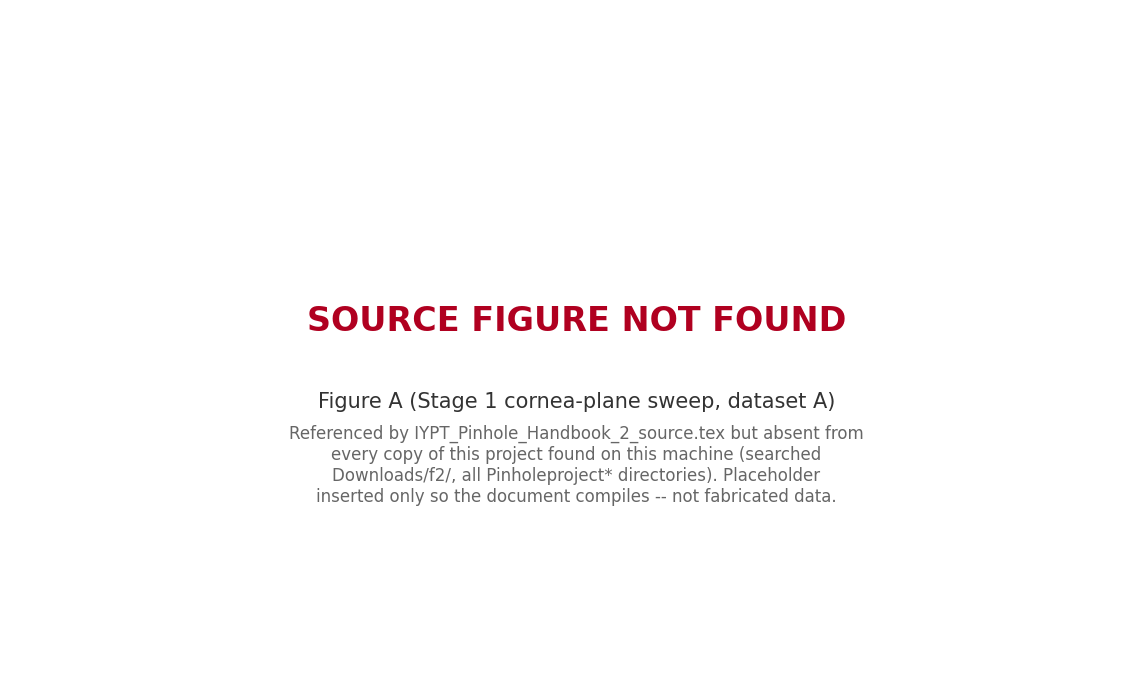
\includegraphics[width=0.85\textwidth]{figs/stage1_cornea_sweep_A.png}
\caption{Stage 1 cornea-plane sweep: peak intensity, $r_{EE}(79\%)$, FWHM radius, and on-axis intensity vs.\ aperture diameter, colored by gap distance (dataset A).}
\label{fig:stage1a}
\end{figure}
\begin{figure}[h!]
\centering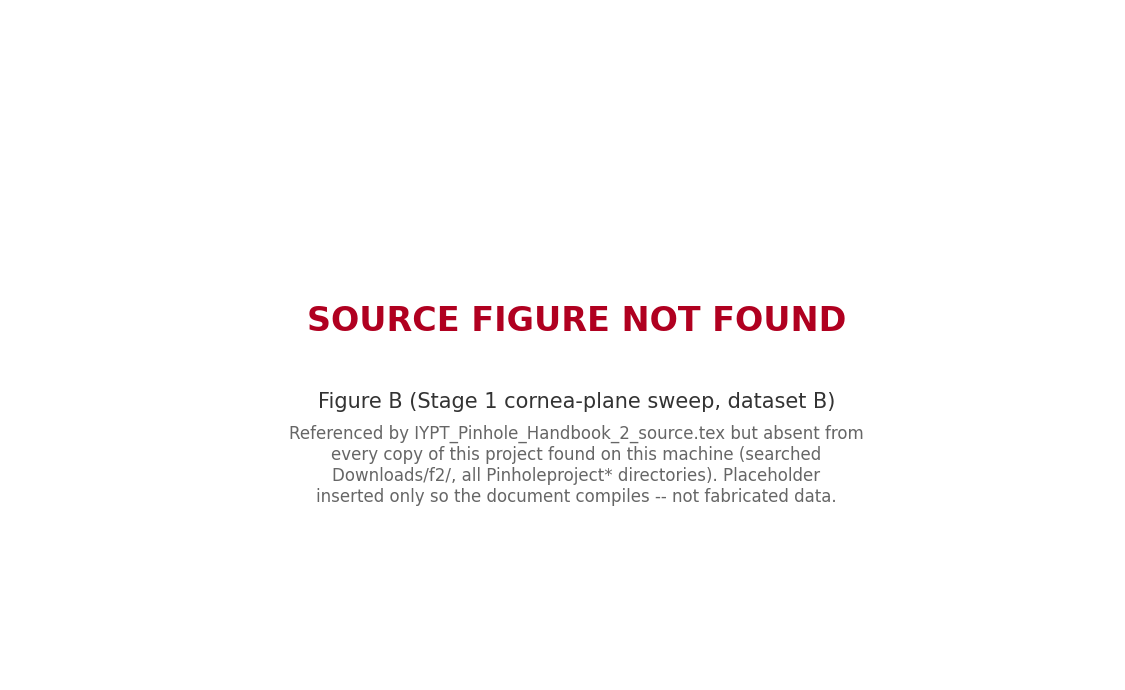
\includegraphics[width=0.85\textwidth]{figs/stage1_cornea_sweep_B.png}
\caption{Stage 1 cornea-plane sweep, dataset B (independent cross-check run).}
\label{fig:stage1b}
\end{figure}

\section{A genuine, expected physical oscillation}
\label{sec:oscillation}
Early analysis found the on-axis and peak intensity curves oscillating sharply as aperture diameter increased at fixed gap. Fitting the classical closed form (Eq.~\ref{eq:onaxis}) against the simulated data gave a correlation of $0.997$ -- confirming genuine Fresnel-zone interference, not numerical noise.

\section{Validation and a resolution-dependent limitation}
A full validation suite checks energy conservation, band-limit adequacy, aperture Nyquist sampling, window-size/wraparound safety, and central-peak-assumption validity. One dataset (grid $N=1024$) failed the energy-conservation check on $100\%$ of rows -- traced to that specific grid resolution being under-resolved relative to the window size, producing aliasing that can masquerade as physically meaningful structure, not a physics error.

\chapter{Stage 2: The Full Eye Model}
\label{ch:stage2}

\section{Architecture: one continuous physical chain}
Stage 2 extends Stage 1 through a single, deliberately narrow bridge module that re-exports exactly the Stage 1 primitives needed, enforcing by import structure (not convention) that no other Stage 2 file ever imports Stage 1 directly. The physical chain: plane wave $\to$ pinhole $\to$ ASM across $\dgap$ $\to$ pupil clipping $\to$ thin-lens phase $\to$ ASM across $\vr$ $\to$ retinal intensity. This is one continuous wave-optics simulation, not two blur-radius numbers added together -- the correct alternative to the deprecated RSS combination (Eq.~\ref{eq:rtotal}).

\section{The axial-length myopia model}
Myopia is modeled via
\begin{equation}
L_{\text{ax}} = \frac{n'}{P_0 - M}, \qquad L_0 = \frac{n'}{P_0}
\label{eq:axialmyopia}
\end{equation}
where $P_0=60$D is held fixed for every degree of myopia $M$, and $n'=1.336$ (vitreous refractive index) by default -- an anatomically-scaled convention, logged explicitly per output row so results are never ambiguous. Only axial length grows; this is the standard clinical model of \emph{axial} myopia, as distinct from a \emph{refractive} model in which power itself would change.

\section{The junction validation gate}
Before propagating a cornea-plane field to the retina, the gate checks: finiteness/non-zero energy, Matsushima band-limit adequacy \emph{at the retina distance} (re-propagating a diagnostic copy of the actual field, rather than assuming the gap-stage window/grid remains adequate at the typically longer retina distance), and a wraparound-safety pre-check using a diffraction-limited minimum-divergence estimate from the cornea field's own second-moment radius (\S\ref{sec:bugfix2}).

\section{Closed-form validation against the Airy disk}
\label{sec:airyvalidation}
At $\dgap=0$ and $M=0$, the full chain reduces exactly to the textbook Fraunhofer setup (Eqs.~\ref{eq:airy}--\ref{eq:encircledenergy}). $r_{EE}(50\%)$ and $r_{EE}(90\%)$ were confirmed to $2\%$ tolerance; $r_{EE}(80\%)$ required an explicitly justified $8\%$ tolerance, since it sits almost exactly at the Airy pattern's first dark ring, where the closed-form curve has zero slope and any small numerical residual is amplified into a much larger radius error -- confirmed empirically across grid sizes $1024$ to $8192$, where an order of magnitude more compute did not reduce this percentile's error below $2.3$--$4.6\%$.

\section{Two real bugs found and fixed}

\subsection{Energy-conservation check was mathematically redundant}
\label{sec:bugfix1}
The original energy-conservation check compared output power against input power at $0.1\%$ tolerance. This was proven identical to the already-separate band-limit-suppression check whenever band-limiting is active: since the transfer function $H$ has unit modulus on every kept propagating order and is exactly zero elsewhere,
\begin{equation}
\varepsilon_{\text{energy}} \equiv \frac{|P_{\text{out}} - P_{\text{in}}|}{P_{\text{in}}} \;=\; f_{\text{suppressed}}
\end{equation}
where $f_{\text{suppressed}}$ is the band-limit-suppressed energy fraction. Confirmed against real sweep data: correlation $1.000000$, mean ratio $1.0$, standard deviation $6\times10^{-14}$. Since the band-limit check's own tolerance ($5\%$) is fifty times looser than the energy check's ($0.1\%$), the energy check was guaranteed to fail on essentially every row -- not from any defect, but from re-flagging already-tolerated, intentional suppression at an unreasonably strict threshold. \textbf{Fix:} test the residual $\varepsilon_{\text{energy}} - f_{\text{suppressed}}$ against the $0.1\%$ tolerance instead, restoring the check's ability to detect an actual defect.

\subsection{The wraparound safety margin was backwards}
\label{sec:bugfix2}
The junction check's pre-lens divergence estimate used $\lambda/(\pi w)$ -- the Gaussian-beam ($M^2=1$) formula for the theoretical \emph{minimum} possible divergence for a beam of second-moment waist $w$. By the standard beam-quality ($M^2$) theorem, this is a lower bound; any non-Gaussian beam, including the Airy-ring-generating field a hard-edged aperture produces, diverges at least as fast. The original docstring called this "conservative (deliberately pessimistic)" -- backwards, since it is a best-case floor, not a worst-case ceiling. \textbf{Fix:} an explicit, documented $\text{margin\_factor}=3.0\times$ inflation, with the docstring corrected to state this is a first-pass compensation, not a validated bound.

\section{R1 sweep result: the true optimum}
\label{sec:r1result}
The project's own initial default sweep ($125$--$200\,\mu$m) reported $r_{EE}(50\%)$ shrinking monotonically -- correctly flagged in the project's own README as evidence the sweep had not yet reached the true minimum, since pure diffraction blur can only decrease monotonically without a competing defocus term. A widened sweep ($75$--$2000\,\mu$m, $550$nm, $12$mm gap) located the true U-shaped minimum:

\begin{table}[h!]
\centering
\caption{R1 sweep result: optimum aperture and minimum blur radius by myopia level.}
\label{tab:r1result}
\begin{tabular}{ccc}
\toprule
Myopia (D) & Optimum aperture $a^*$ ($r_{EE}$ 50\%) & Min.\ blur radius ($\mu$m) \\
\midrule
1 & 300 & 23.04 \\
2 & 300 & 22.65 \\
3 & 300 & 22.29 \\
4 & 300 & 21.99 \\
5 & 400 & 20.83 \\
6 & 400 & 19.79 \\
8 & 400 & 18.16 \\
\bottomrule
\end{tabular}
\end{table}

\chapter{Stage 3a: Brightness-Constrained Optimum Aperture}
\label{ch:stage3a}

\section{The hypothesis under test}
The $300$--$400\,\mu$m blur-only optimum sits below the verified clinical/commercial range of $0.94$--$1.75$mm (Review of Optometry, citing a dedicated clinical study; \S\ref{sec:clinicalbracket}). Rather than treating this as evidence the diffraction physics was wrong, the specific hypothesis tested: does the gap close once retinal brightness -- entirely absent from the pure blur-minimizing objective -- is added as a constraint?

\section{The illuminance model}
\label{sec:illuminancemodel}
For a single circular aperture directly in front of the eye:
\begin{equation}
\Erel = \left(\frac{\min(\ahole, \Dpupil)}{\Dpupil}\right)^2
\label{eq:erel}
\end{equation}
Deliberately distinct from the array photometry formula (Eq.~\ref{eq:photometryarray}). This follows directly from energy conservation: diffraction redistributes power spatially but does not destroy it, so illuminance must be computed from the raw physical aperture area, not any diffraction-broadened spot-size estimate.

\section{Constrained optimization and the headline result}
\label{sec:stage3aresult}
\begin{equation}
a^{*}_{\text{practical}}(M,\Tmin) = \operatorname*{arg\,min}_{\ahole\,:\,\Erel(\ahole)\ge\Tmin} r_{EE}(50\%)
\end{equation}
At $\Tmin=0$ this exactly reproduces Stage 2's original unconstrained result.

\begin{table}[h!]
\centering
\caption{Constrained optimum vs.\ brightness floor $\Tmin$.}
\label{tab:tminresult}
\begin{tabular}{ccc}
\toprule
Brightness floor $\Tmin$ & Constrained optimum $a^*$ & Position vs.\ clinical bracket \\
\midrule
$0\%$ (unconstrained) & $300$--$400\,\mu$m & below \\
$1\%$ & $400\,\mu$m & below \\
$3\%$ & $700\,\mu$m & below \\
$6.25\%$ & $1000\,\mu$m & \textbf{inside} \\
$9\%$ & $1250\,\mu$m & \textbf{inside} \\
$12.25\%$ & $1500\,\mu$m & upper edge \\
\bottomrule
\end{tabular}
\end{table}

A brightness floor of roughly $6$--$9\%$ of full natural-pupil illuminance -- physically modest, comparable to ordinary sunglass tinting -- moves the optimum from $300$--$400\,\mu$m into the verified clinical bracket, uniformly across every myopia level tested.

\begin{figure}[h!]
\centering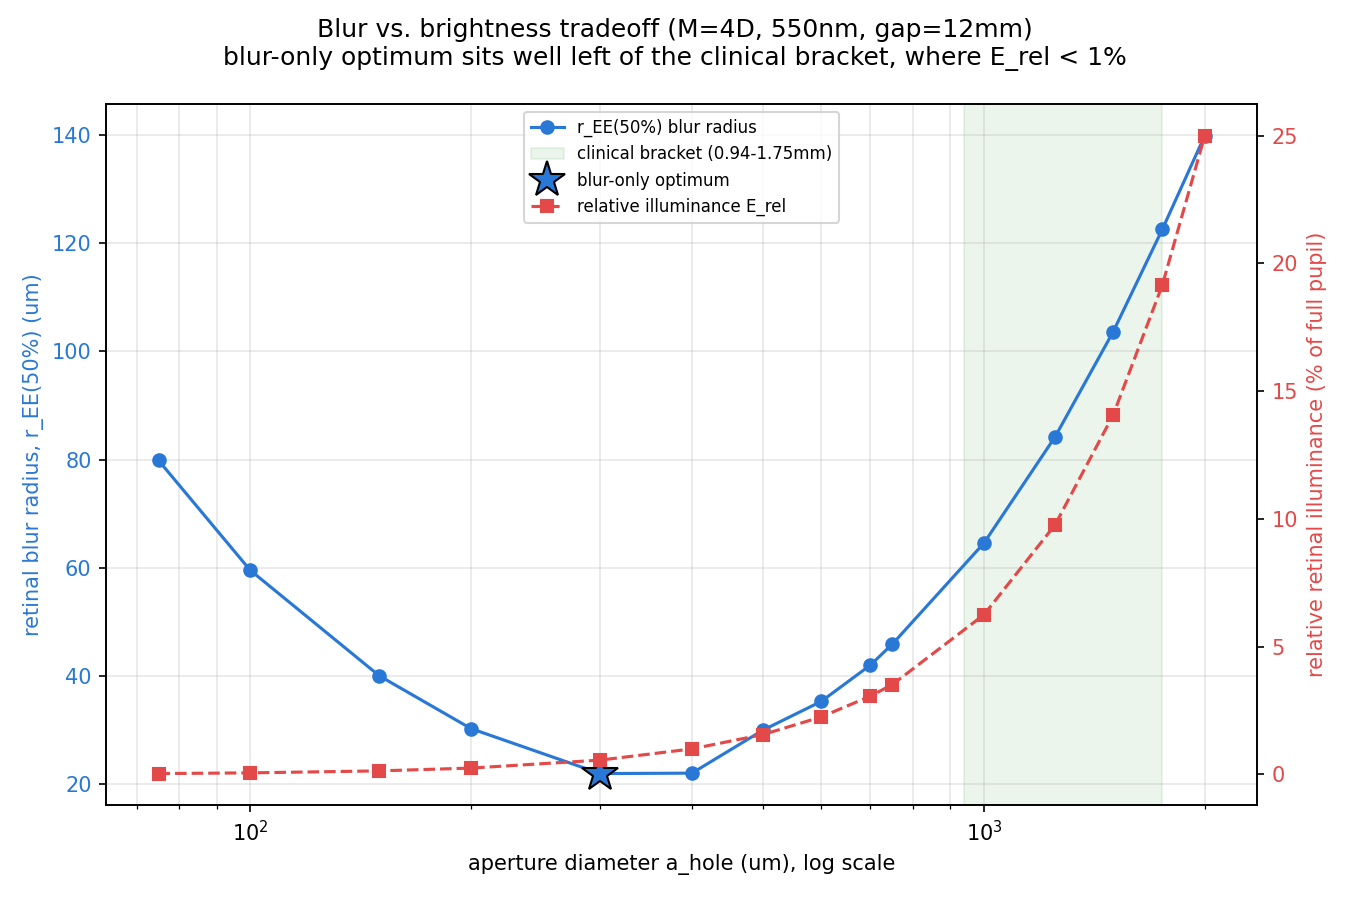
\includegraphics[width=0.85\textwidth]{figs/stage3a_fig1_blur_vs_brightness.png}
\caption{Blur radius (left axis) and relative retinal illuminance (right axis) vs.\ aperture, $M=4$D.}
\end{figure}
\begin{figure}[h!]
\centering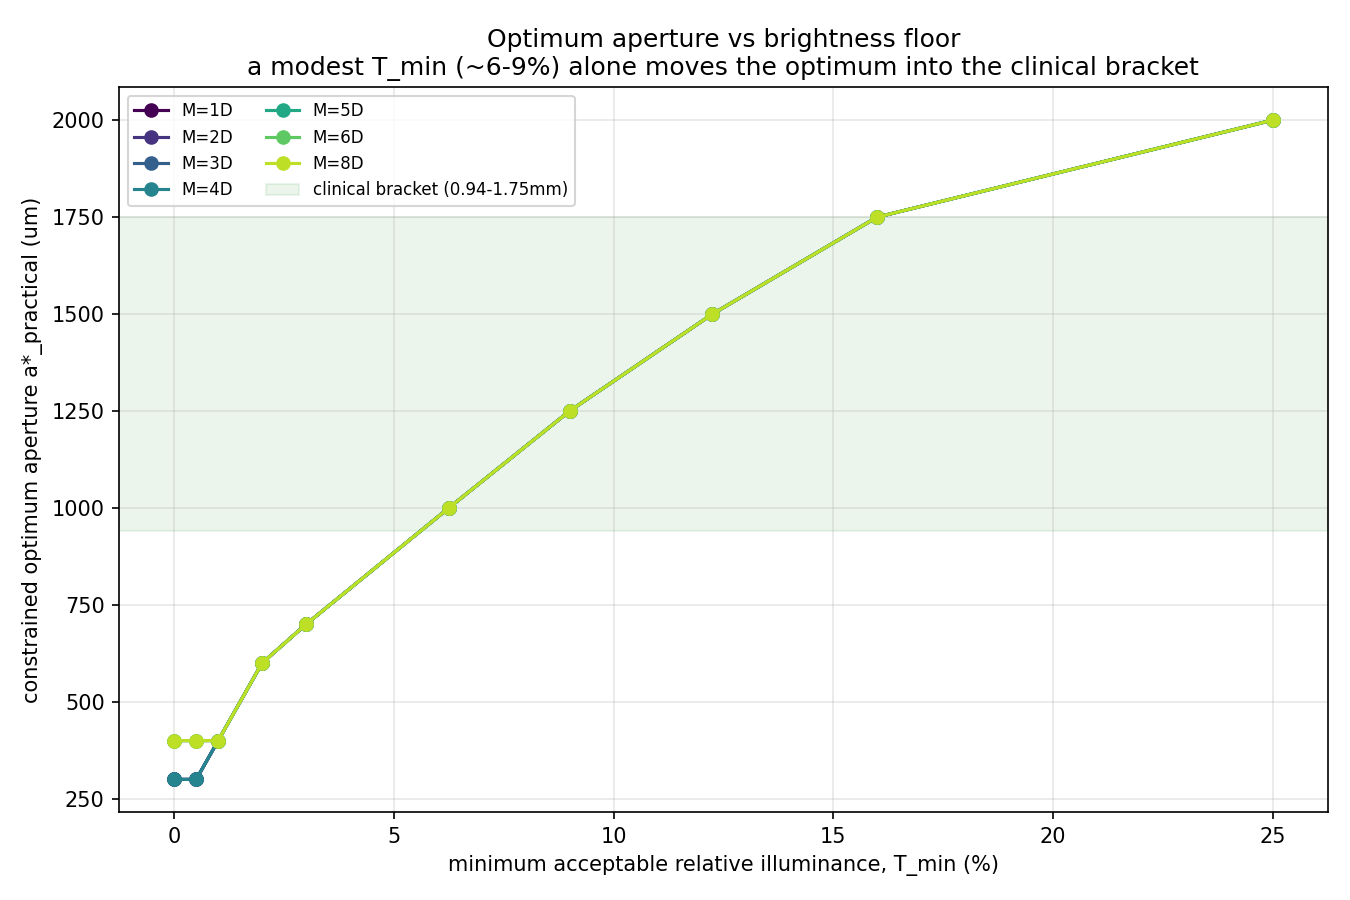
\includegraphics[width=0.85\textwidth]{figs/stage3a_fig2_optimum_vs_Tmin.png}
\caption{Constrained optimum aperture vs.\ brightness floor $\Tmin$, all myopia levels. Green band: verified clinical bracket.}
\end{figure}
\begin{figure}[h!]
\centering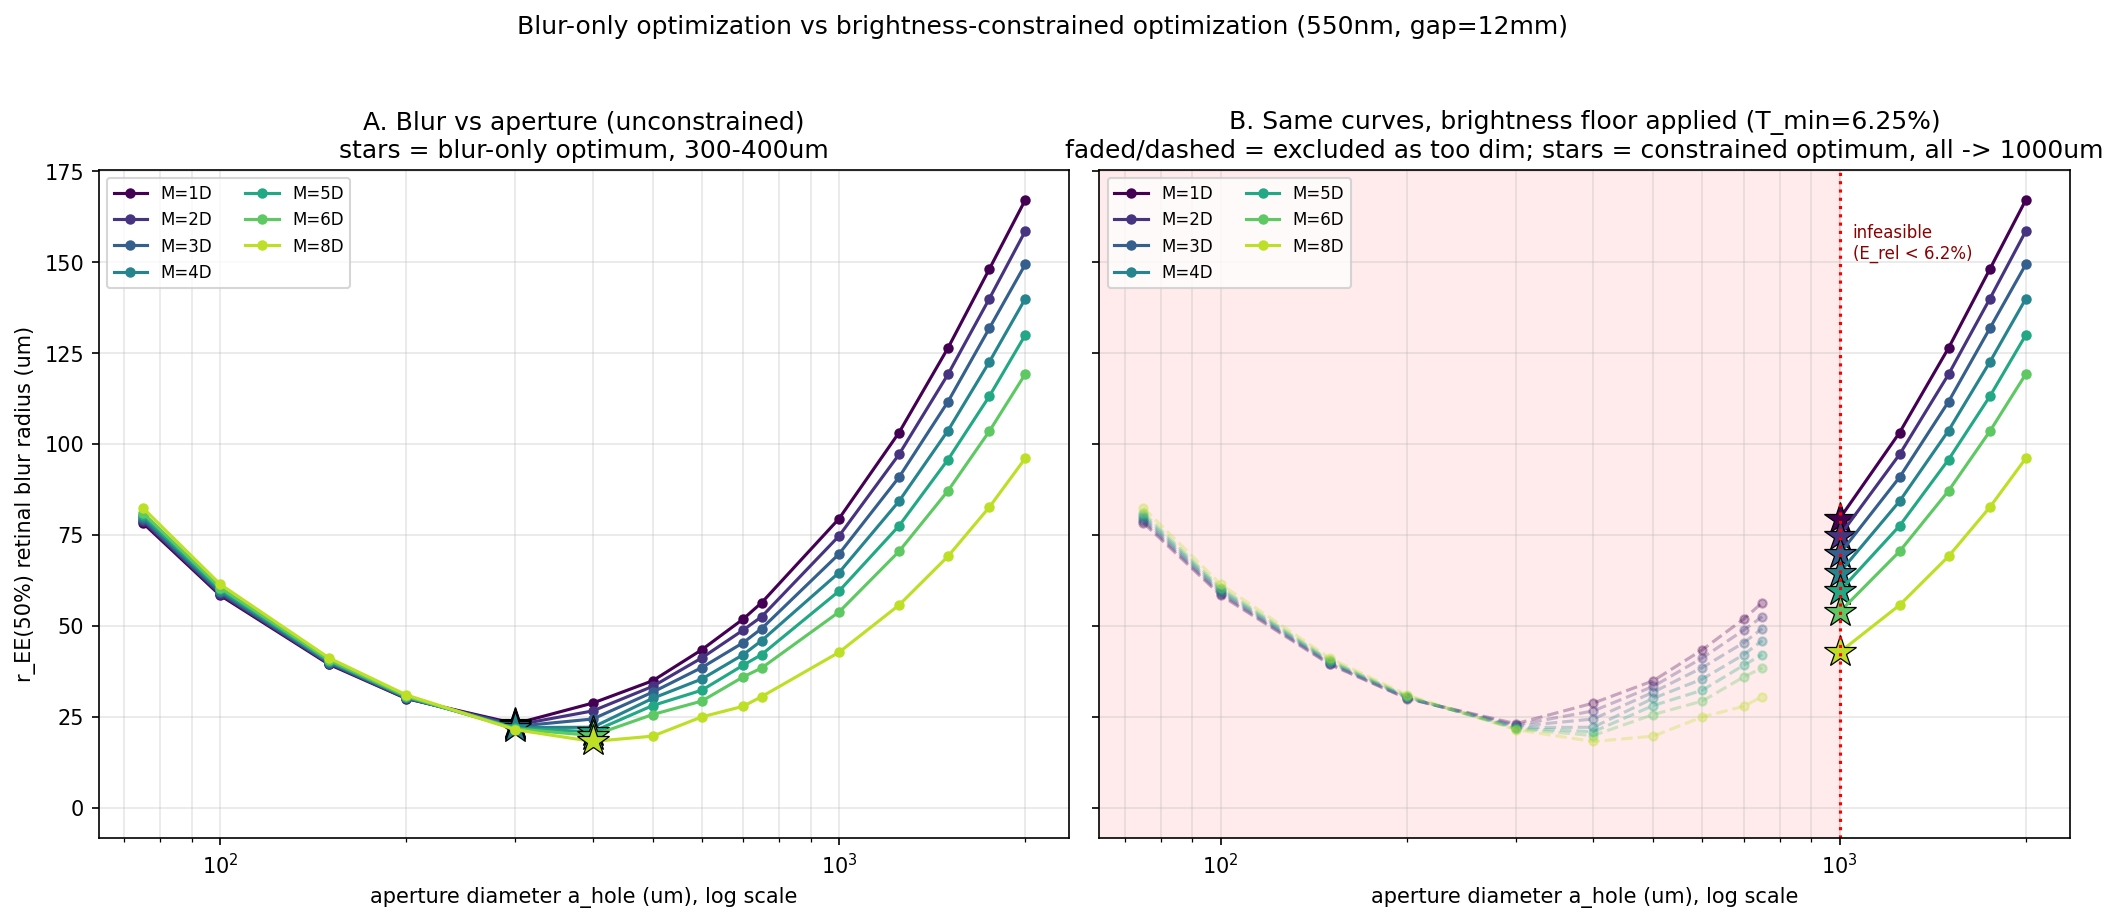
\includegraphics[width=0.85\textwidth]{figs/stage3a_fig4_blur_then_constraint.png}
\caption{Panel A: unconstrained blur-vs-aperture curves. Panel B: same curves with the $6.25\%$ brightness floor applied.}
\end{figure}

\section{What this result does and does not establish}
This establishes that the \emph{size} of the gap is fully explainable in magnitude by a physically plausible brightness constraint. It does \emph{not} establish that $6$--$9\%$ is the true physiological threshold -- that number was found by matching the known clinical range, not derived independently from a cited illuminance-acuity relationship. Stated explicitly as an open item (\S\ref{sec:openitems}).

\section{Percentile-choice robustness check}
\label{sec:convergence}
$r_{EE}(70\%)$ was computed for the first time (extracted directly from the raw retinal field, no Stage 2 modification) and combined with the pre-existing $80\%/90\%$ columns.

\begin{figure}[h!]
\centering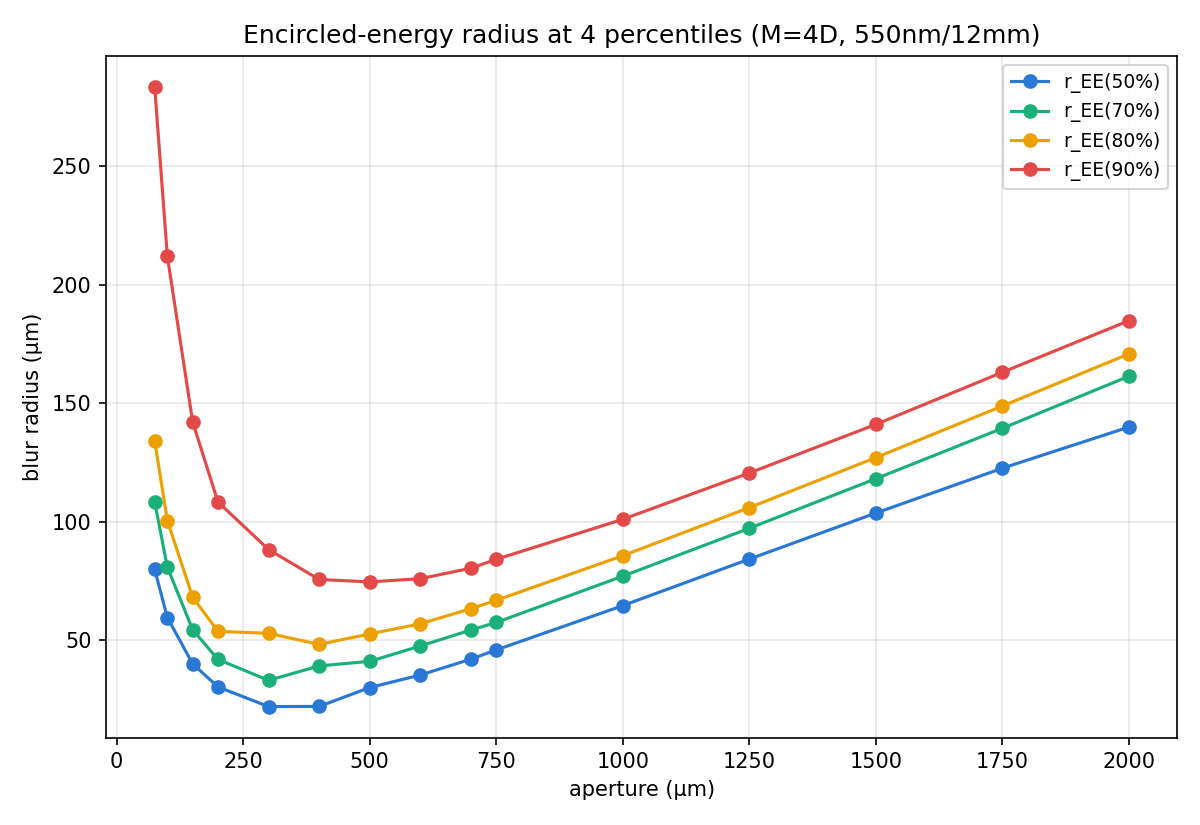
\includegraphics[width=0.8\textwidth]{figs/ee_all_percentiles.png}
\caption{$r_{EE}$ at $50/70/80/90\%$ vs.\ aperture, $M=4$D.}
\end{figure}

Unconstrained, the four percentiles disagree modestly ($300$--$400\,\mu$m for $50/70\%$, $400$--$600\,\mu$m for $80/90\%$). Once the $6.25\%$ brightness floor is applied, \textbf{all four percentiles converge to exactly the same answer -- $1000\,\mu$m -- at every myopia level}. Once the illuminance floor forces the aperture past the point where every percentile's blur curve is simultaneously increasing, the constraint boundary dominates rather than the metric choice: \textbf{the brightness floor matters far more than which encircled-energy percentile is chosen.}

\chapter{Stage 3 Human Vision: Comprehensive Metric Suite}
\label{ch:stage3hv}

\section{Design principle: citation discipline}
\label{sec:literature-discipline}
This stage's citation database classifies every implemented relationship as \emph{first\_principles} (needs no citation, e.g.\ energy conservation, the Fourier-optics definition of MTF), \emph{published} (a specific named model, with any simplification stated), or \emph{heuristic} (a simplified stand-in, e.g.\ where the full multi-parameter Barten CSF model could not be reproduced exactly). Twenty citation entries cover the Strehl ratio, MTF/OTF, the Airy diameter, F-number, RMS spot radius, the troland unit and CIE photopic luminous efficacy, two CSF parametrizations, the Rose--DeVries law, Weber contrast, the Blackwell (1946) dataset, MAR/Snellen conversion, the Visual Strehl metric, the Stiles--Crawford effect, and ocular aberration magnitudes.

\section{Photometric chain}
The full chain from scene luminance to photon flux at the retina:
\begin{equation}
E_{\text{retina}} = \frac{\pi N \tau}{4\,(\text{F\#})^2} \cdot L_{\text{scene}}
\label{eq:retinalirradiance}
\end{equation}
(the standard image-irradiance camera equation, reusing this project's own F-number function). A default scene luminance of $10{,}000\text{ cd/m}^2$ and heuristic ocular transmission $\tau=0.90$ (stated range $0.85$--$0.95$) are both exposed as overridable arguments, not hardcoded silently.

\begin{figure}[h!]
\centering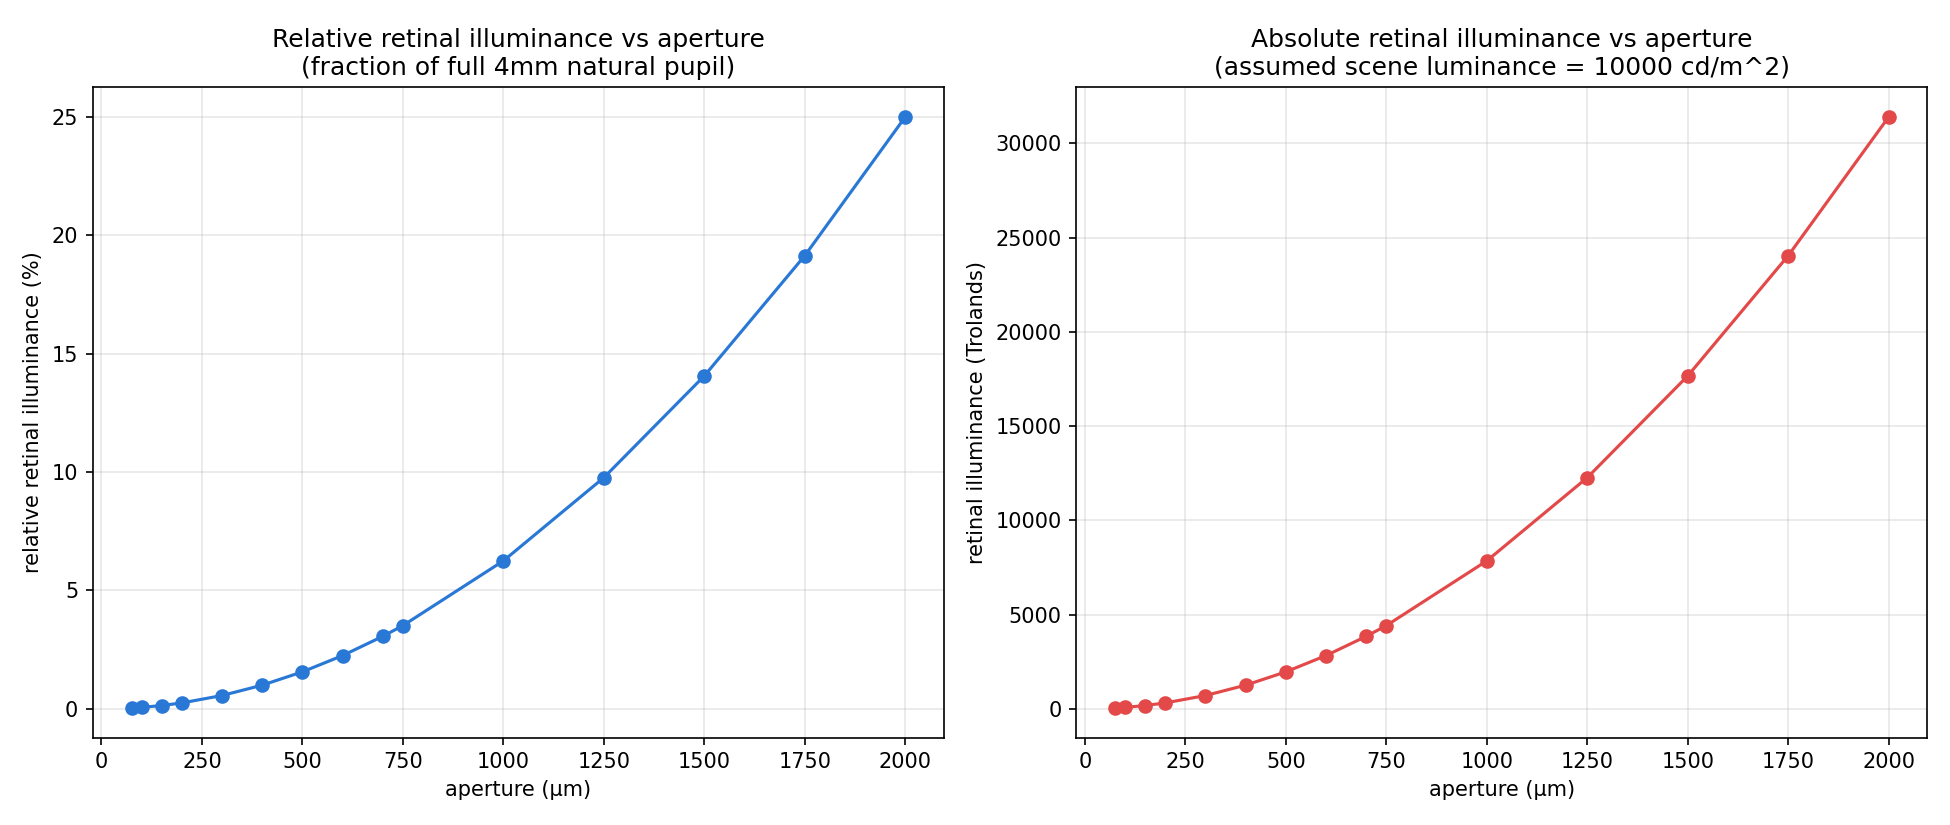
\includegraphics[width=0.85\textwidth]{figs/illuminance_troland.png}
\caption{Relative retinal illuminance (left) and absolute Trolands at the stated assumed scene luminance (right), vs.\ aperture, $M=4$D.}
\end{figure}

\section{MTF, OTF, and two contrast-sensitivity models}
\label{sec:mtfcsf}
MTF is computed as $|\mathcal{F}\{\text{PSF}\}|$ (Eq.~\ref{eq:mtfotf}), normalized to DC and radially averaged -- exact, no free parameters. Two published CSF parametrizations are implemented and deliberately never merged: a simplified band-pass model peaking near $4$ cycles/degree, and the Mannos--Sakrison parametrization peaking near $8$ cycles/degree. The genuine disagreement between these published peak locations is reported as a finding, not resolved by picking one.

\begin{figure}[h!]
\centering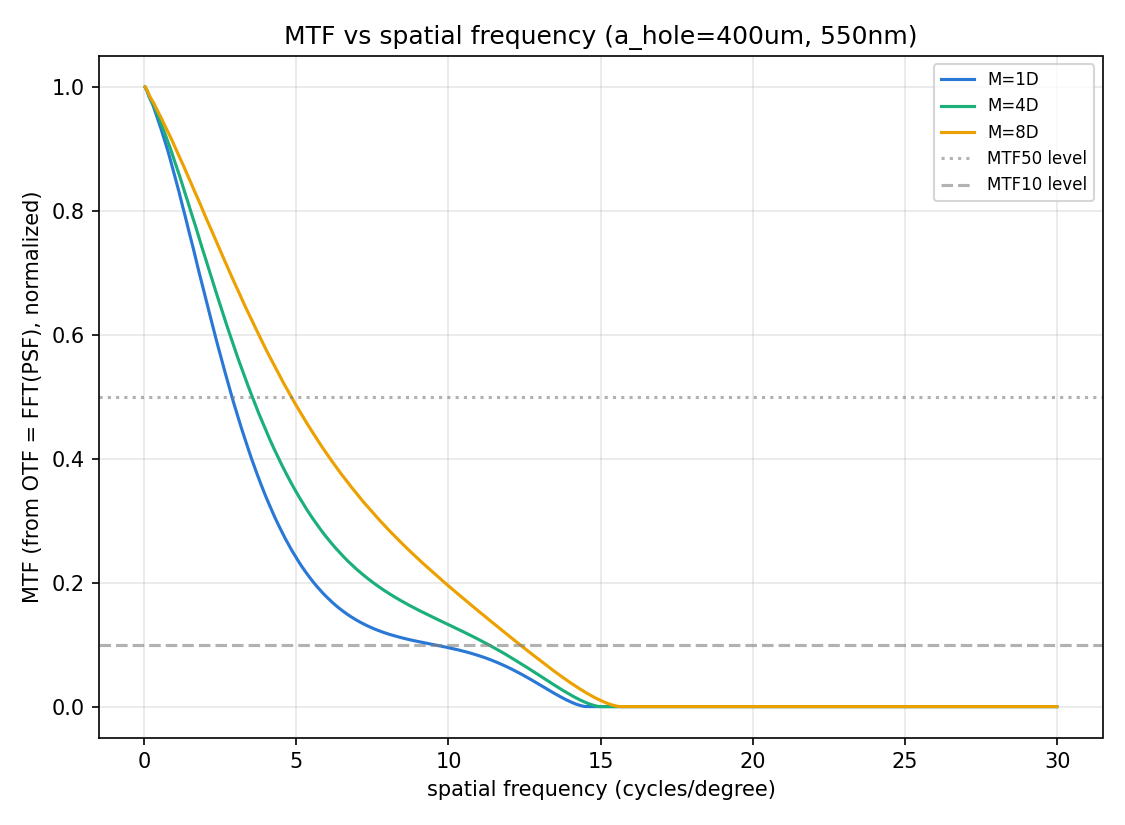
\includegraphics[width=0.85\textwidth]{figs/mtf_curves.png}
\caption{Radially-averaged MTF vs.\ spatial frequency, three myopia levels, with MTF50/MTF10 levels marked.}
\end{figure}
\begin{figure}[h!]
\centering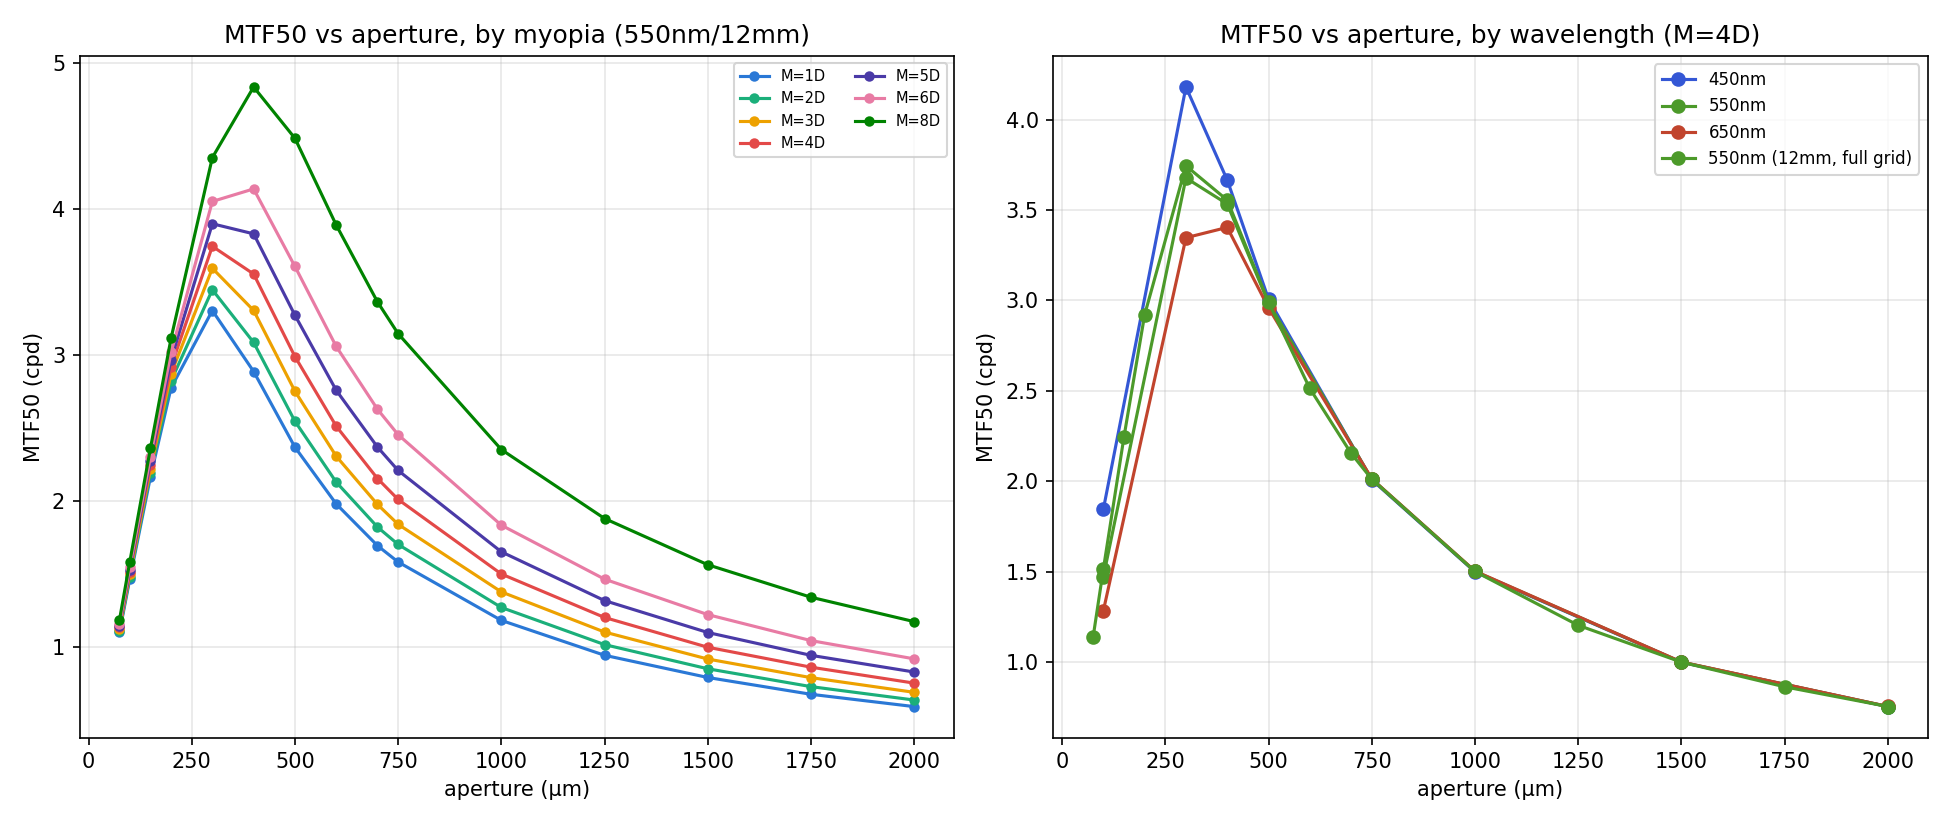
\includegraphics[width=0.85\textwidth]{figs/mtf50_extended.png}
\caption{MTF50 vs.\ aperture, by myopia level (left) and by wavelength at $M=4$D (right).}
\end{figure}
\begin{figure}[h!]
\centering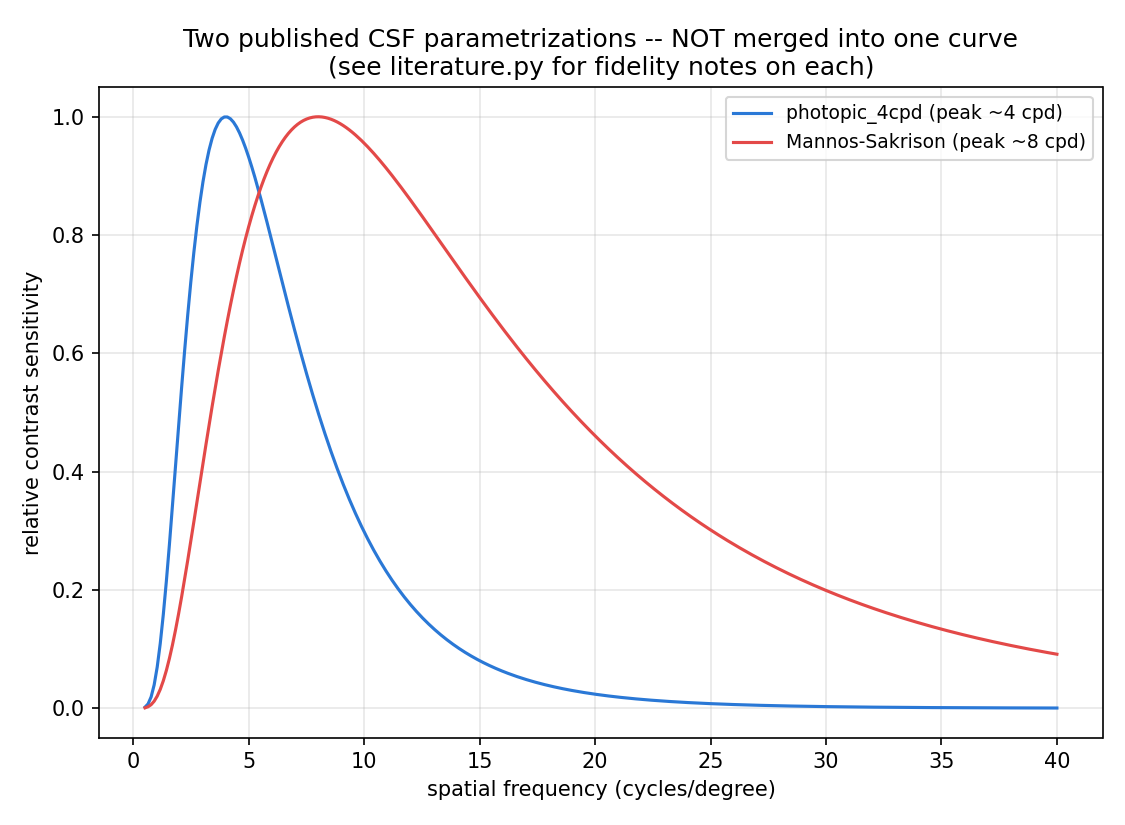
\includegraphics[width=0.7\textwidth]{figs/csf_comparison.png}
\caption{Two independently published CSF parametrizations, plotted together, showing the genuine peak-location disagreement.}
\end{figure}

\section{Three independent visual-acuity prediction models}
(1) MAR/Snellen from the MTF50 or MTF10 cutoff via the exact identity that a resolvable grating of $C$ cycles/degree corresponds to
\begin{equation}
\text{MAR (arcmin)} = \frac{30}{C}
\label{eq:marfromC}
\end{equation}
(2) an approximate Visual Strehl (VSX-style) metric, CSF-weighting both actual and diffraction-limited MTF before comparing areas; (3) a Rose--DeVries photon-noise-limited SNR bound, where resolvable detail scales as
\begin{equation}
\text{MAR} \propto \Phi^{-1/2}
\label{eq:rosedevries}
\end{equation}
with $\Phi$ relative photon flux, calibrated to report a \emph{relative} change in the noise floor, not an absolute clinical prediction.

\begin{figure}[h!]
\centering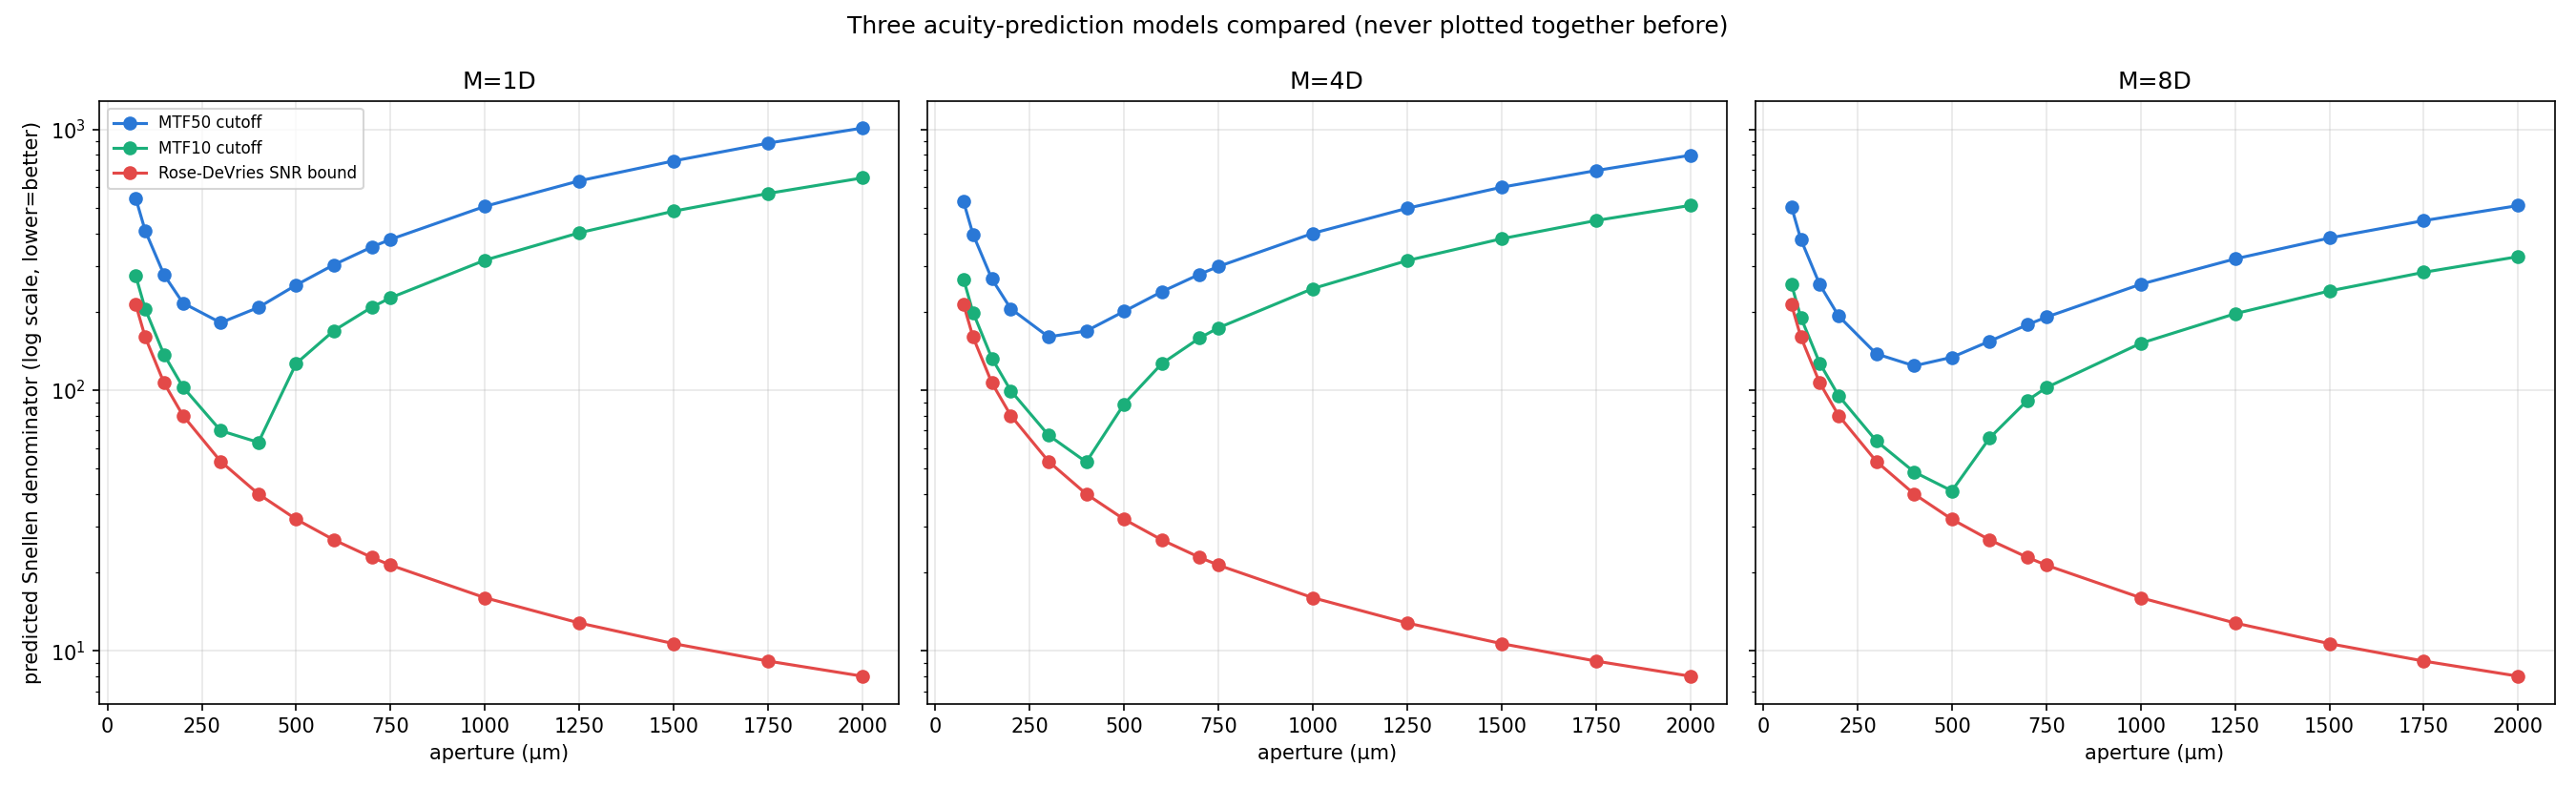
\includegraphics[width=0.95\textwidth]{figs/acuity_models_combined.png}
\caption{All three acuity-prediction models, per myopia level ($M=1,4,8$D) -- the combined comparison that did not exist before this stage.}
\end{figure}

\section{Strehl ratio and Pareto-optimal trade-off analysis}
Strehl ratio,
\begin{equation}
S = \frac{I_{\text{peak,actual}}}{I_{\text{peak,diffraction-limited}}}
\label{eq:strehl}
\end{equation}
with the Mar\'echal criterion ($S \ge 0.8$ for "diffraction-limited") cited as context. Multi-objective Pareto-front analysis treats blur radius (minimize) and throughput (maximize) as competing objectives.

\section{Full-chain validation}
Reuses the Airy-disk gate (\S\ref{sec:airyvalidation}); the initial error-budget scaffold logs, contributor by contributor, whether each unmodeled effect is quantified or left as a qualitative note (extended in \S\ref{sec:errorbudget}).

\chapter{Stage 3 Integrated: Cross-Validation and Two Confirmed Anomalies}
\label{ch:stage3int}

\section{One shared grid, not two datasets stitched together}
Before combining, Stage 3a's and Stage 3 Human Vision's independent illuminance formulas were confirmed to agree \emph{exactly} at four test points ($75,400,1200,4000\,\mu$m) before standardizing on the latter. The merge asserts exactly $105$ rows ($15$ apertures $\times$ $7$ myopia levels), raising an error rather than silently truncating on mismatch, and generalizes the brightness-constrained optimum search to all ten metrics this project has produced.

\section{Extended sweeps}
\label{sec:extendedsweeps}
Three supplementary sweeps: (1) retina-plane FWHM across the full grid, reapplying Stage 1's validated algorithm at the retina plane for the first time; (2) a tenfold finer aperture sweep at $M=4,8$D specifically to test the Strehl non-monotonicity; (3) a representative $450/650$nm and $15$mm-gap extension on an $8$-aperture subset, deliberately scoped down from the full grid.

\section{Confirmed anomaly 1: retina-plane FWHM ring-hopping}
\label{sec:anomaly1}
Stage 1's own FWHM ring-hopping bug (fixed at the cornea plane) reappears at the retina plane, never previously tested there: FWHM jumps from $4.7\,\mu$m to $154.7\,\mu$m between two adjacent $250$-micron-spaced test apertures at $M=4$D -- a factor of over $30$. \textbf{Retina-plane FWHM should not be treated as a reliable single-value metric for this system.}

\begin{figure}[h!]
\centering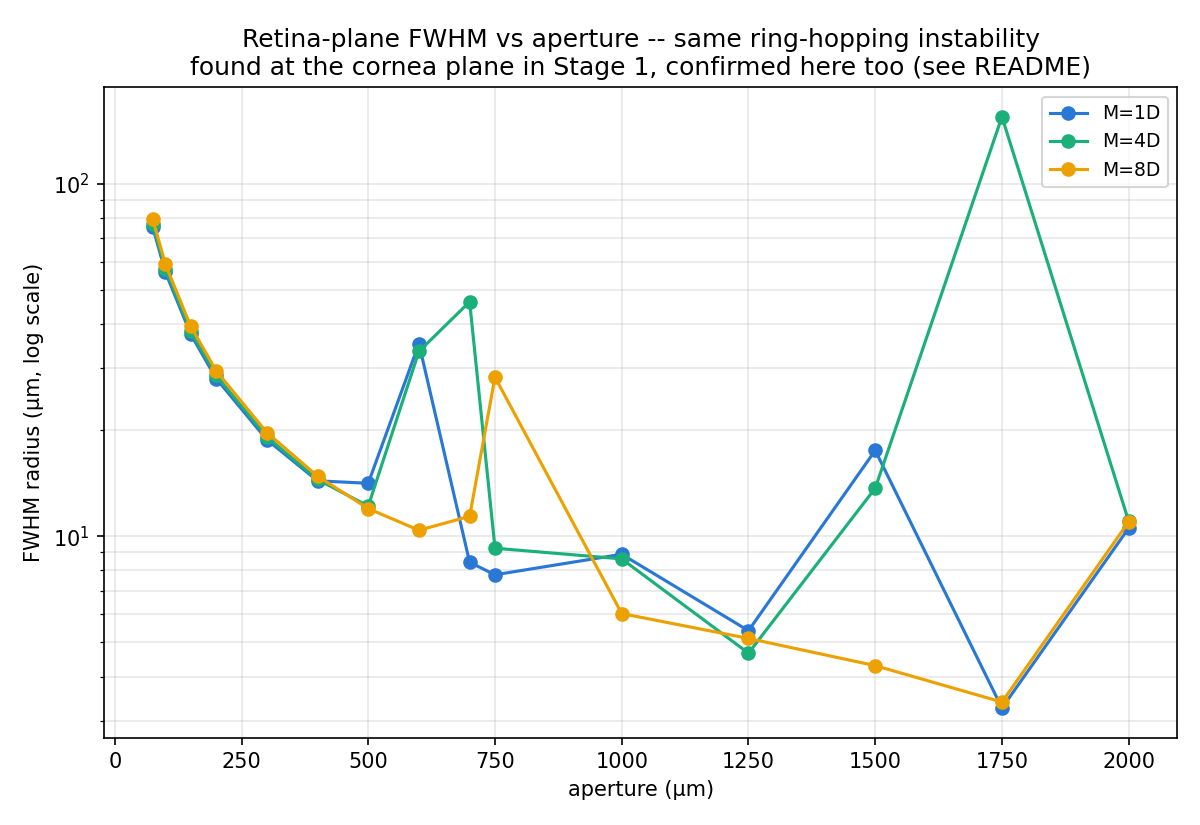
\includegraphics[width=0.85\textwidth]{figs/retina_fwhm_ring_hopping.png}
\caption{Retina-plane FWHM vs.\ aperture (log scale), confirming the ring-hopping instability.}
\end{figure}

\section{Confirmed anomaly 2: Strehl non-monotonicity is genuine}
\label{sec:anomaly2}
The coarse sweep's Strehl-maximizing aperture jumped non-monotonically across myopia levels. The tenfold finer sweep resolved this: rather than smoothing into one peak, it revealed \emph{more} local maxima ($6$--$7$, not fewer) and \emph{larger} swings (up to $8.4\times$, not smaller) -- the opposite of a discretization artifact. \textbf{Strehl ratio is not a reliable single-peak optimization target for this system at these scales.}

\begin{figure}[h!]
\centering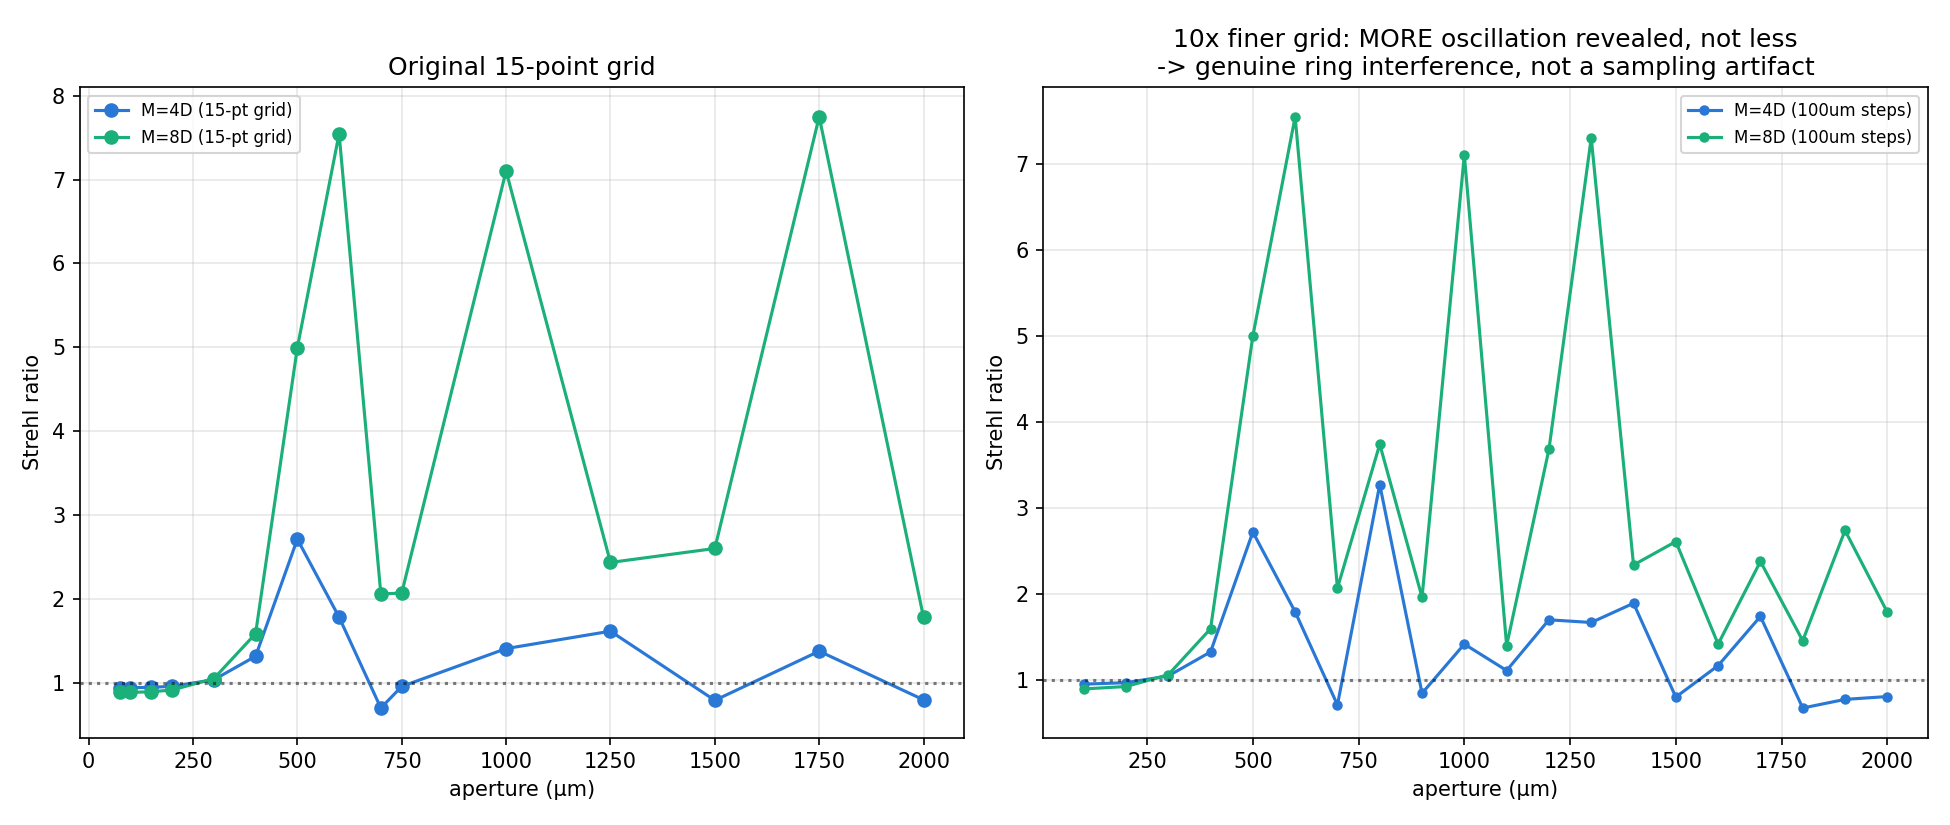
\includegraphics[width=0.85\textwidth]{figs/strehl_investigation.png}
\caption{Strehl ratio at $15$-point (left) vs.\ tenfold-finer $100\,\mu$m-step (right) resolution -- the finer grid reveals \emph{more} oscillation.}
\end{figure}

\section{Sensitivity heatmaps}
\begin{figure}[h!]
\centering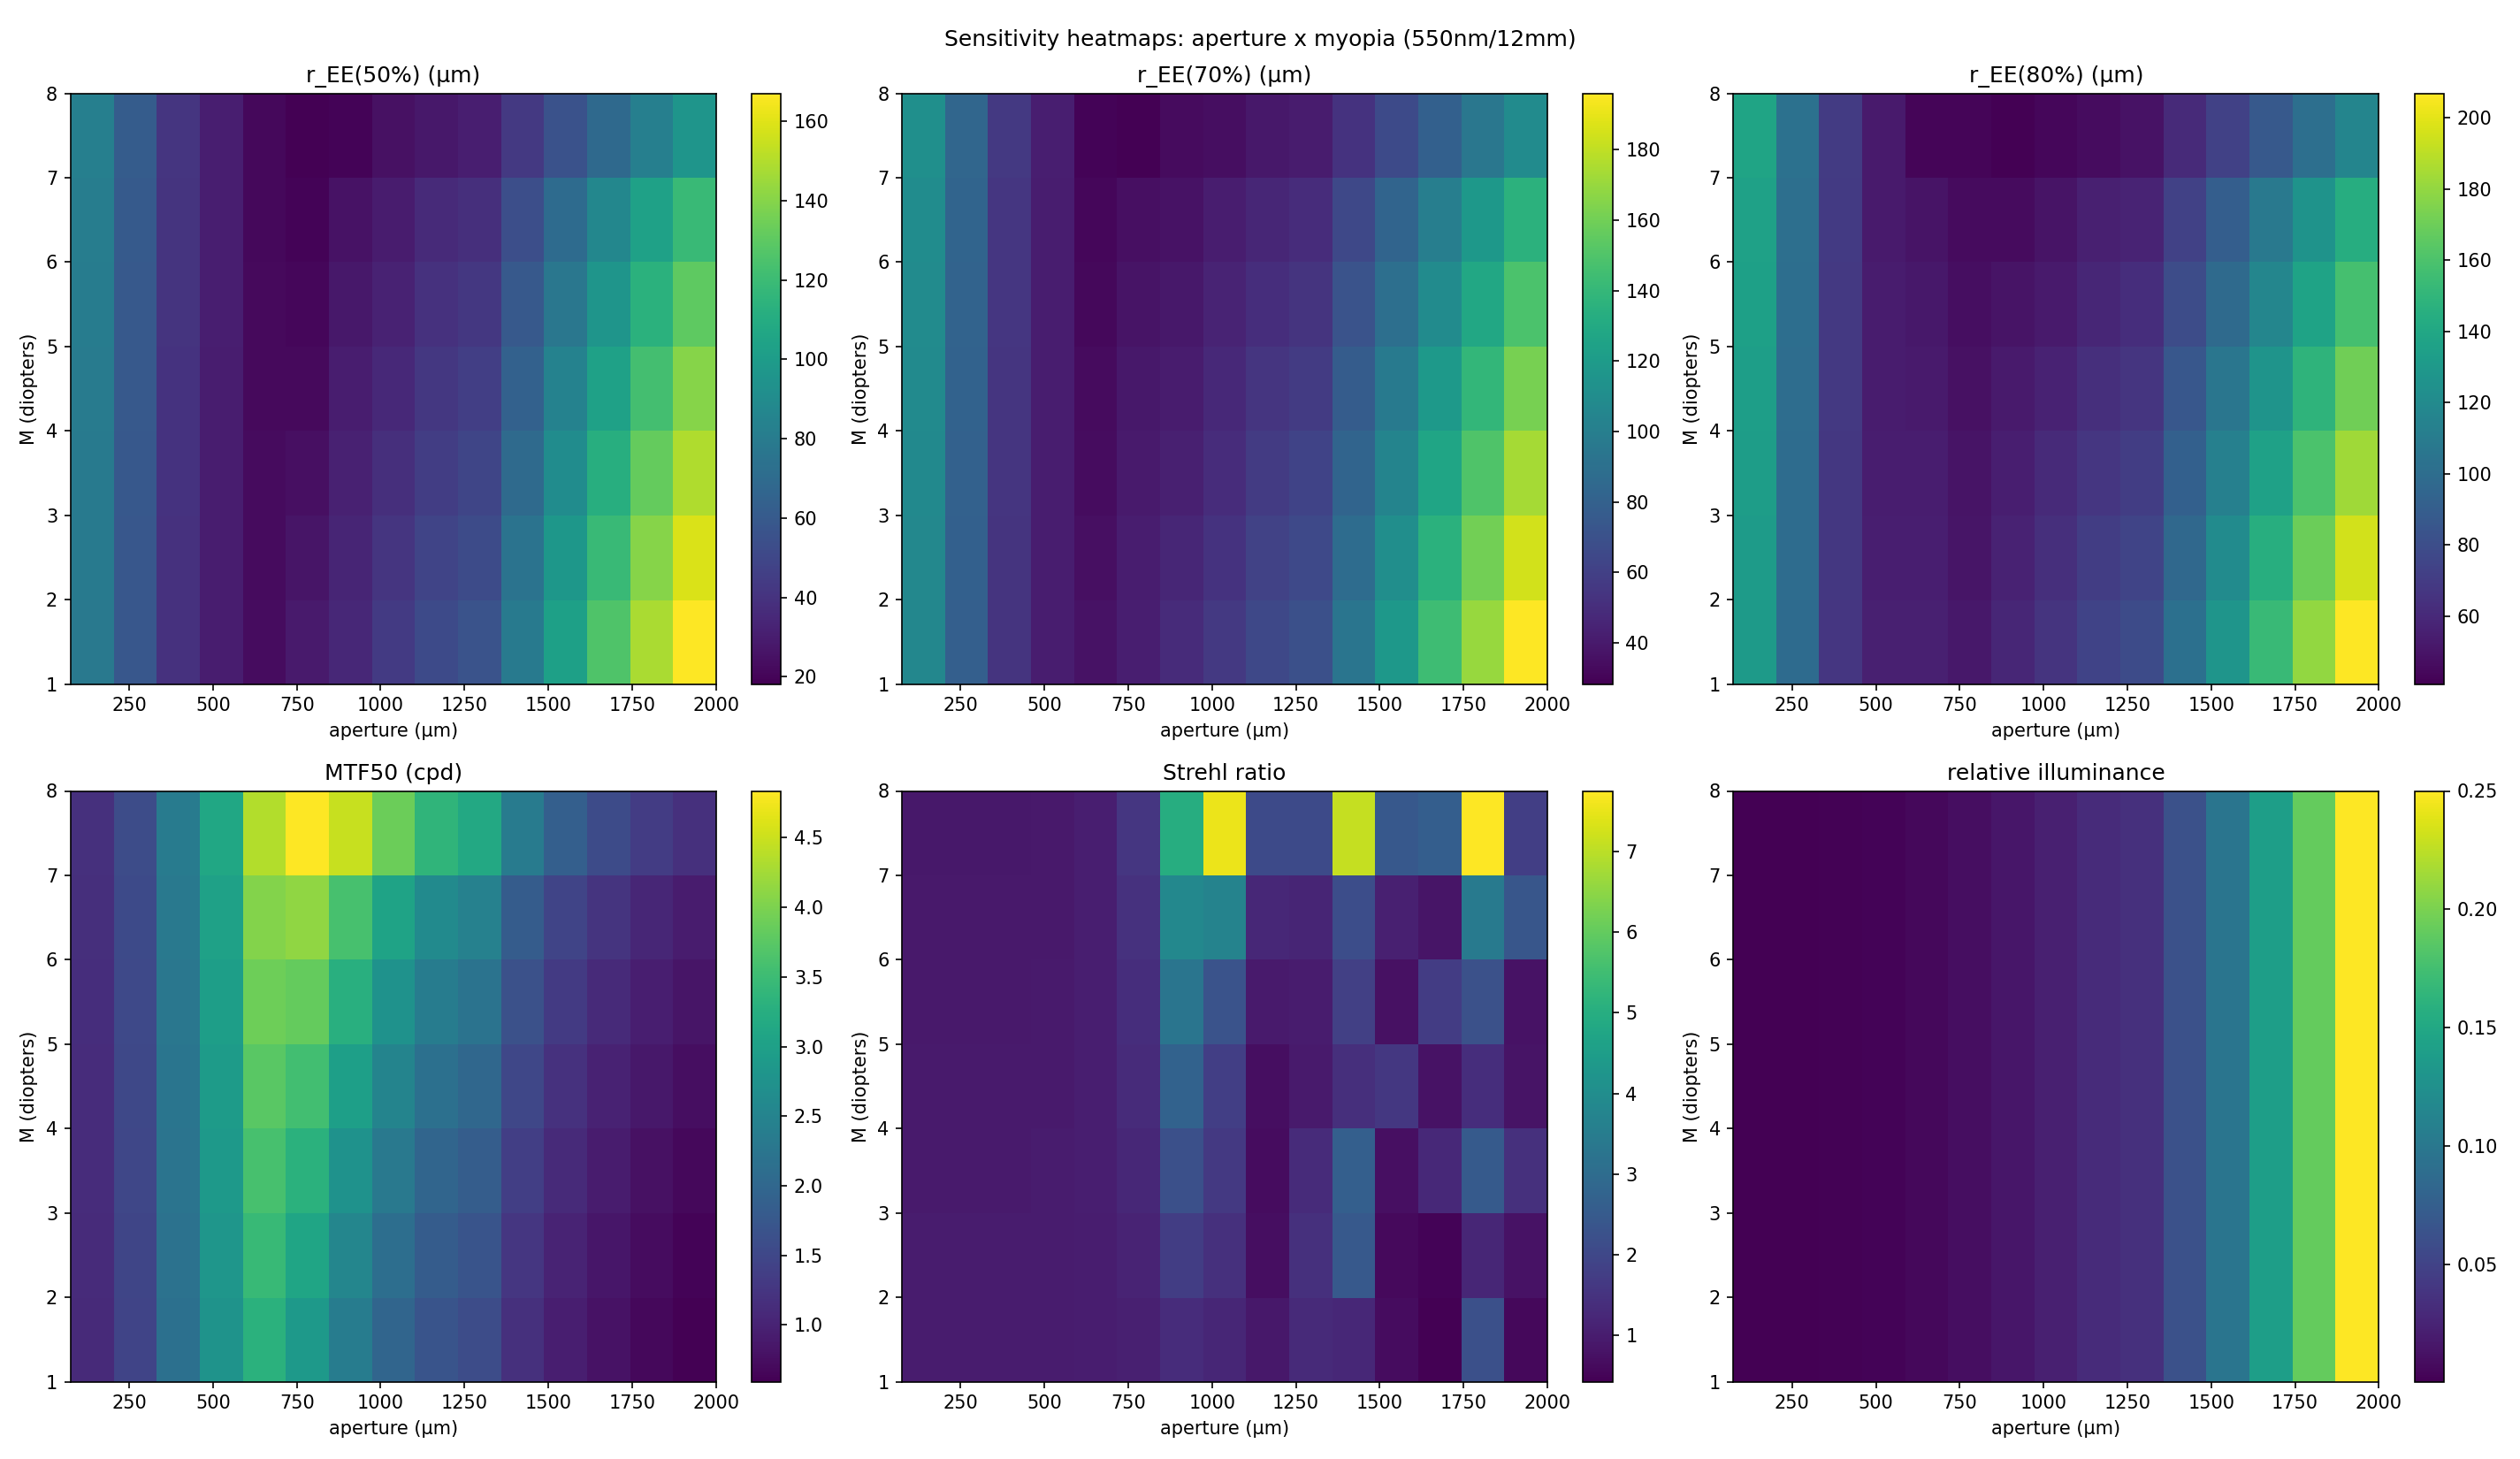
\includegraphics[width=0.95\textwidth]{figs/sensitivity_heatmaps_aperture_M.png}
\caption{Sensitivity heatmaps: aperture vs.\ myopia, for $r_{EE}(50\%)$, MTF50, Strehl, and relative illuminance.}
\end{figure}
\begin{figure}[h!]
\centering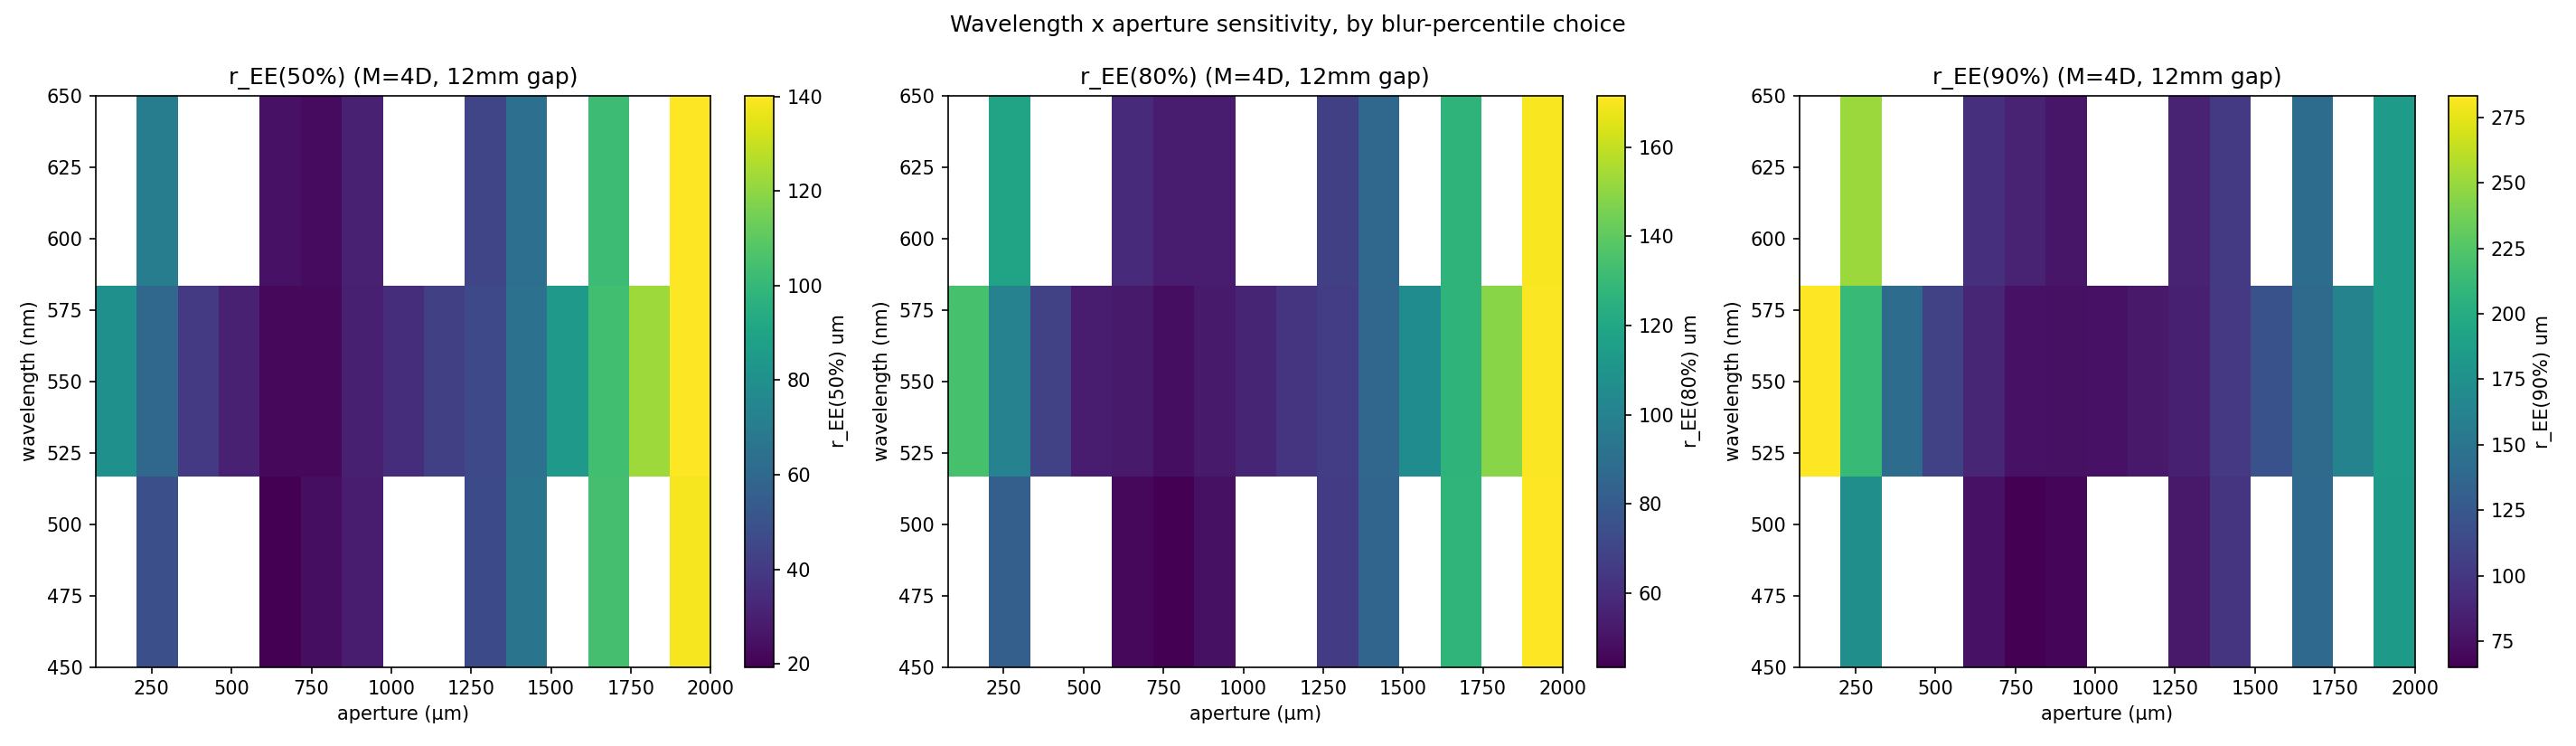
\includegraphics[width=0.75\textwidth]{figs/sensitivity_heatmap_wavelength_aperture.png}
\caption{$r_{EE}(50\%)$ sensitivity: wavelength vs.\ aperture at $M=4$D.}
\end{figure}

\section{Extended validation with visible tolerance bands}
\begin{figure}[h!]
\centering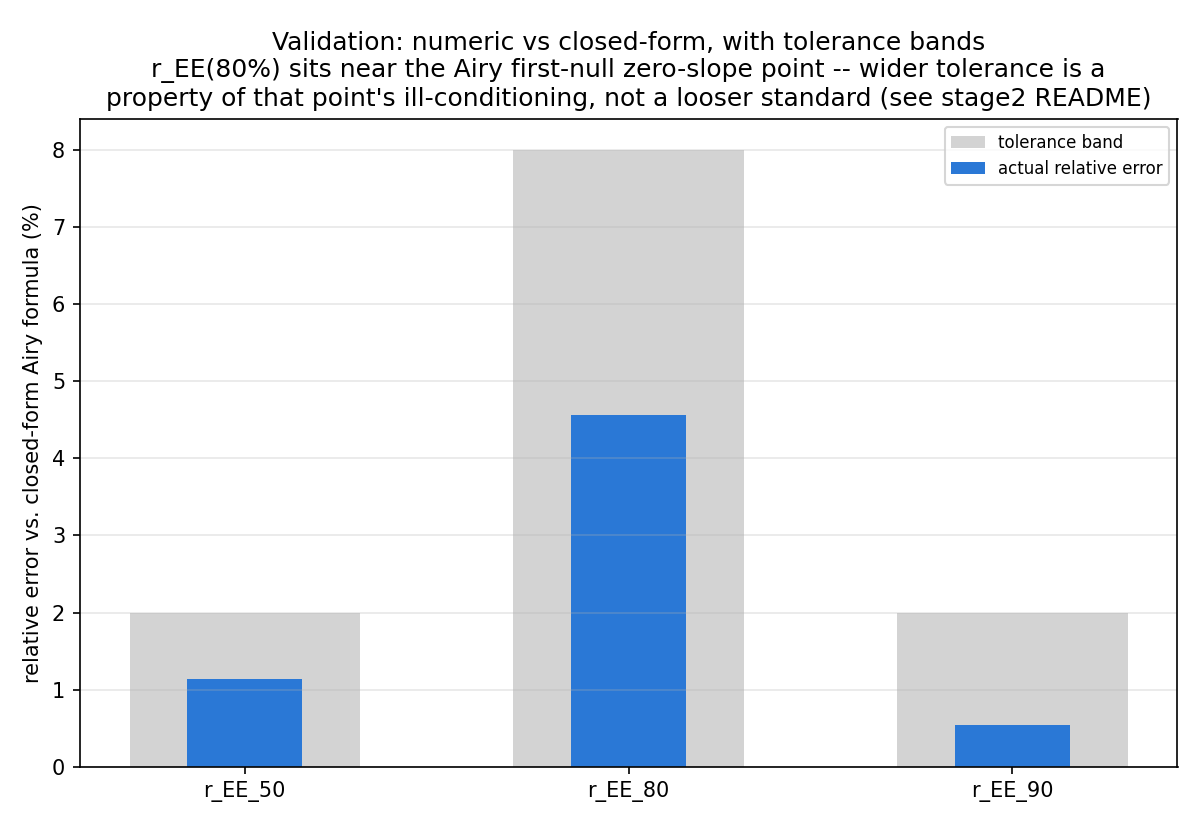
\includegraphics[width=0.85\textwidth]{figs/validation_tolerance_bands.png}
\caption{Numeric vs.\ closed-form Airy result, with explicit tolerance bands per percentile.}
\end{figure}

\section{Pareto fronts across the full myopia range}
\begin{figure}[h!]
\centering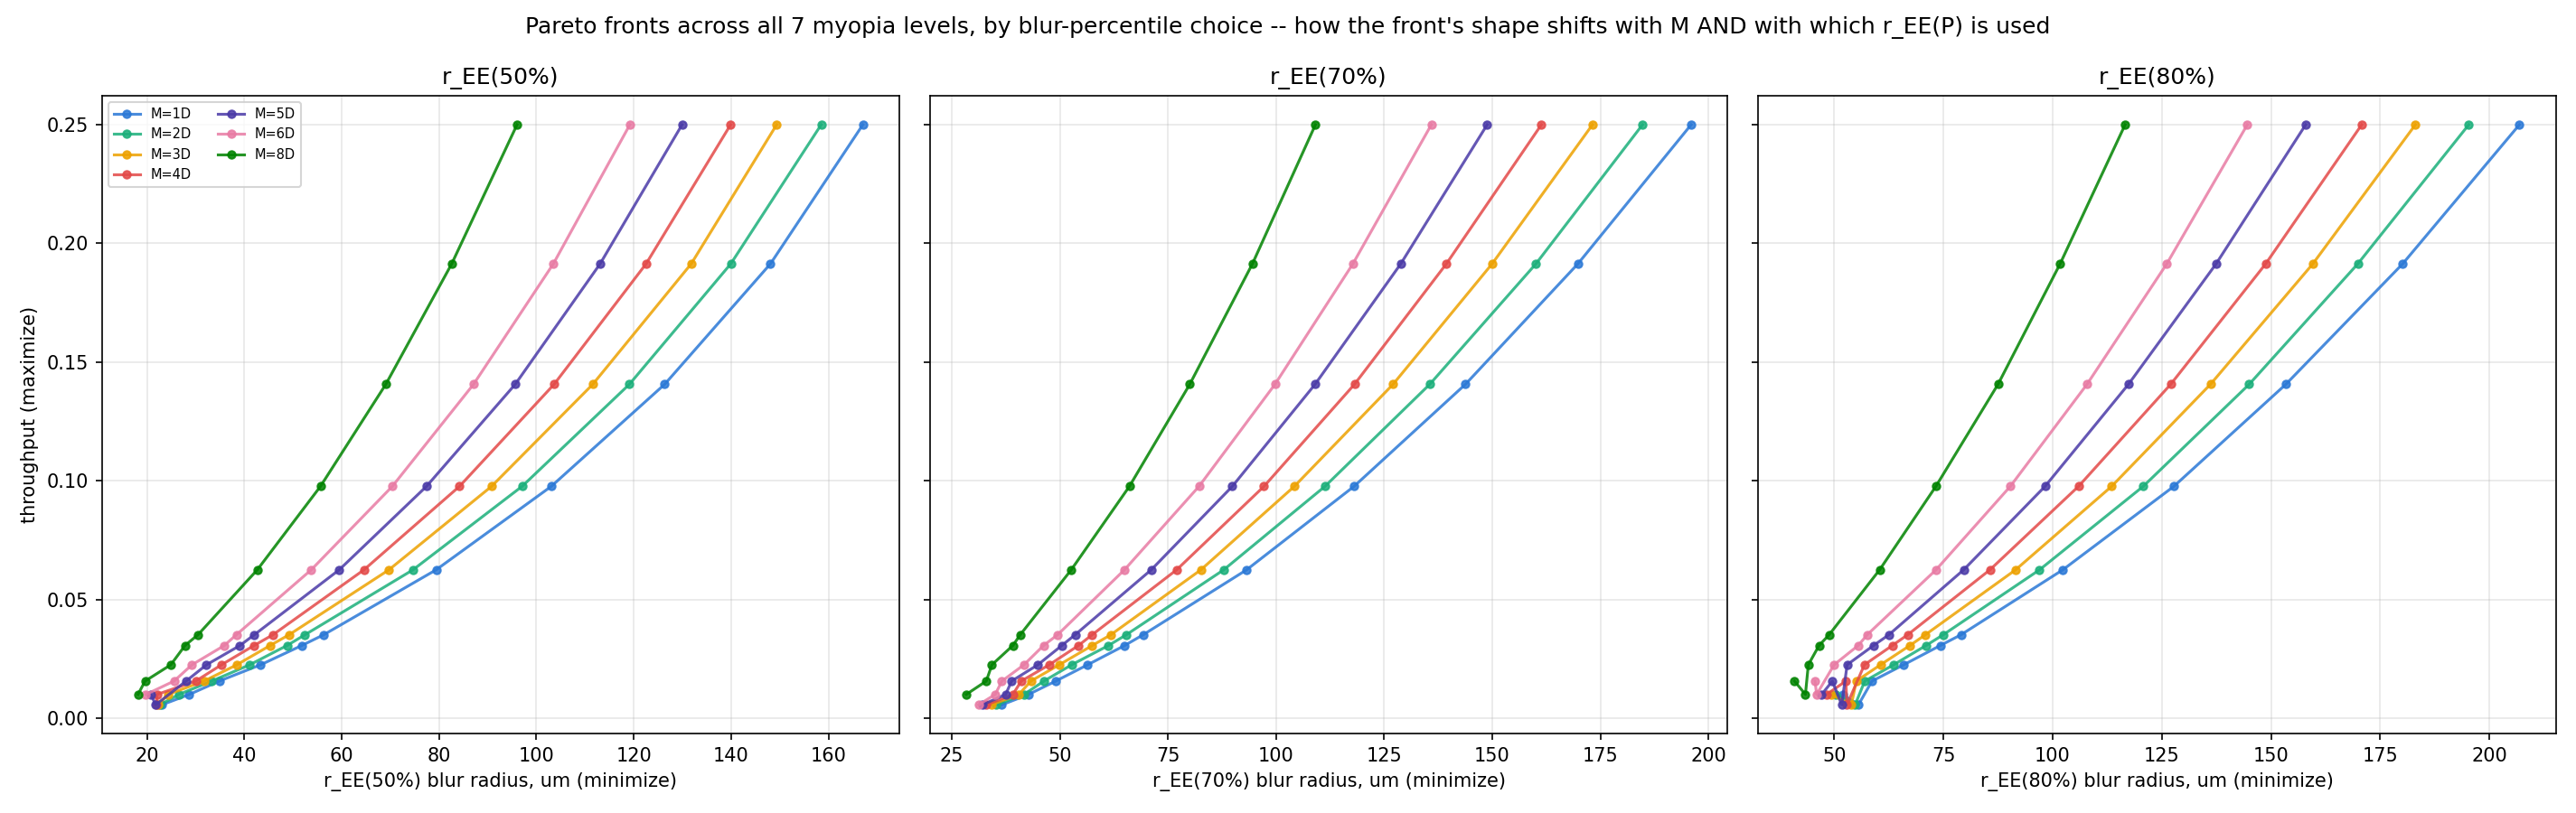
\includegraphics[width=0.85\textwidth]{figs/pareto_all_M_overlay.png}
\caption{Pareto-optimal fronts (blur radius vs.\ throughput) overlaid across all seven tested myopia levels.}
\end{figure}

\chapter{Model Comparison: Why the Numbers Disagree, Diagnosed Three Ways}
\label{ch:comparison}

This chapter documents the single most important synthesis result in this handbook: an independent audit comparing three implementations against each other and against real-world reference data, concluding that the different "optimum aperture" figures across this project's history, the deprecated closed-form formulas, real clinical literature, and real patents disagree for three distinct, individually diagnosed reasons -- not because any one model is simply broken.

\section{The three models compared}
\begin{table}[h!]
\centering
\caption{Three compared models: basis and scope.}
\begin{tabular}{p{2cm}p{7cm}p{3cm}}
\toprule
Model & What it computes & Basis \\
\midrule
1 & Exact ASM, pinhole to cornea only. No eye, no myopia. & \texttt{stage1\_v2} \\
2 & Exact ASM $\times 2$ + lens phase: full chain with axial myopia. & \texttt{stage2} \\
3 & The deprecated closed-form chain: $\aeff$, $\rgeo/\rdiff/\rtotal$ (RSS), $a^*$. Pure algebra. & \texttt{classical\_formulas.py} \\
\bottomrule
\end{tabular}
\end{table}

\section{Finding 1 --- the old formula's accuracy depends entirely on which stage it is applied at}
\label{sec:finding1}
\begin{table}[h!]
\centering
\caption{Divergence of the deprecated formula vs.\ exact numerical result.}
\begin{tabular}{lcc}
\toprule
Comparison & Mean divergence & Max divergence \\
\midrule
Cornea: $\aeff/2$ vs.\ Model 1's exact $r_{EE}(80\%)$ & $13.8\%$ & $23.7\%$ \\
Retina: $\rtotal$ vs.\ Model 2's exact $r_{EE}(50\%)$ & $64.8\%$ & $192.8\%$ \\
\bottomrule
\end{tabular}
\end{table}

$\aeff$ was designed as a cornea-plane spot-size estimate, and there it tracks the exact result reasonably well (Fig.~\ref{fig:comp-cornea}) -- consistently $14$--$24\%$ high, same overall shape. The much larger failure occurs when the same formula family is repurposed for retina-blur optimization via RSS -- exactly the step the reference handbooks call physically wrong (Figs.~\ref{fig:comp-m1}--\ref{fig:comp-m8}).

\begin{figure}[h!]
\centering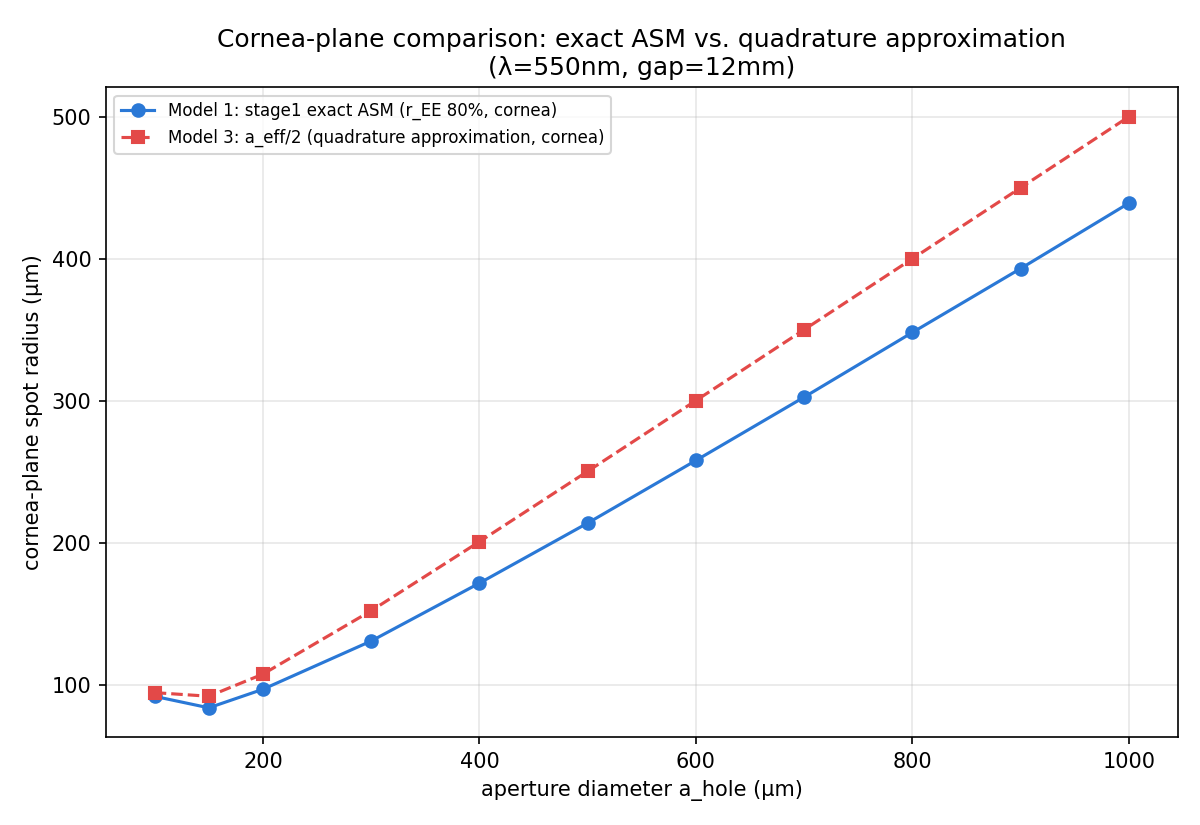
\includegraphics[width=0.8\textwidth]{figs/comparison_cornea.png}
\caption{Cornea-plane: old $\aeff/2$ vs.\ exact $r_{EE}(80\%)$. Consistently biased high but correct in shape.}
\label{fig:comp-cornea}
\end{figure}
\begin{figure}[h!]
\centering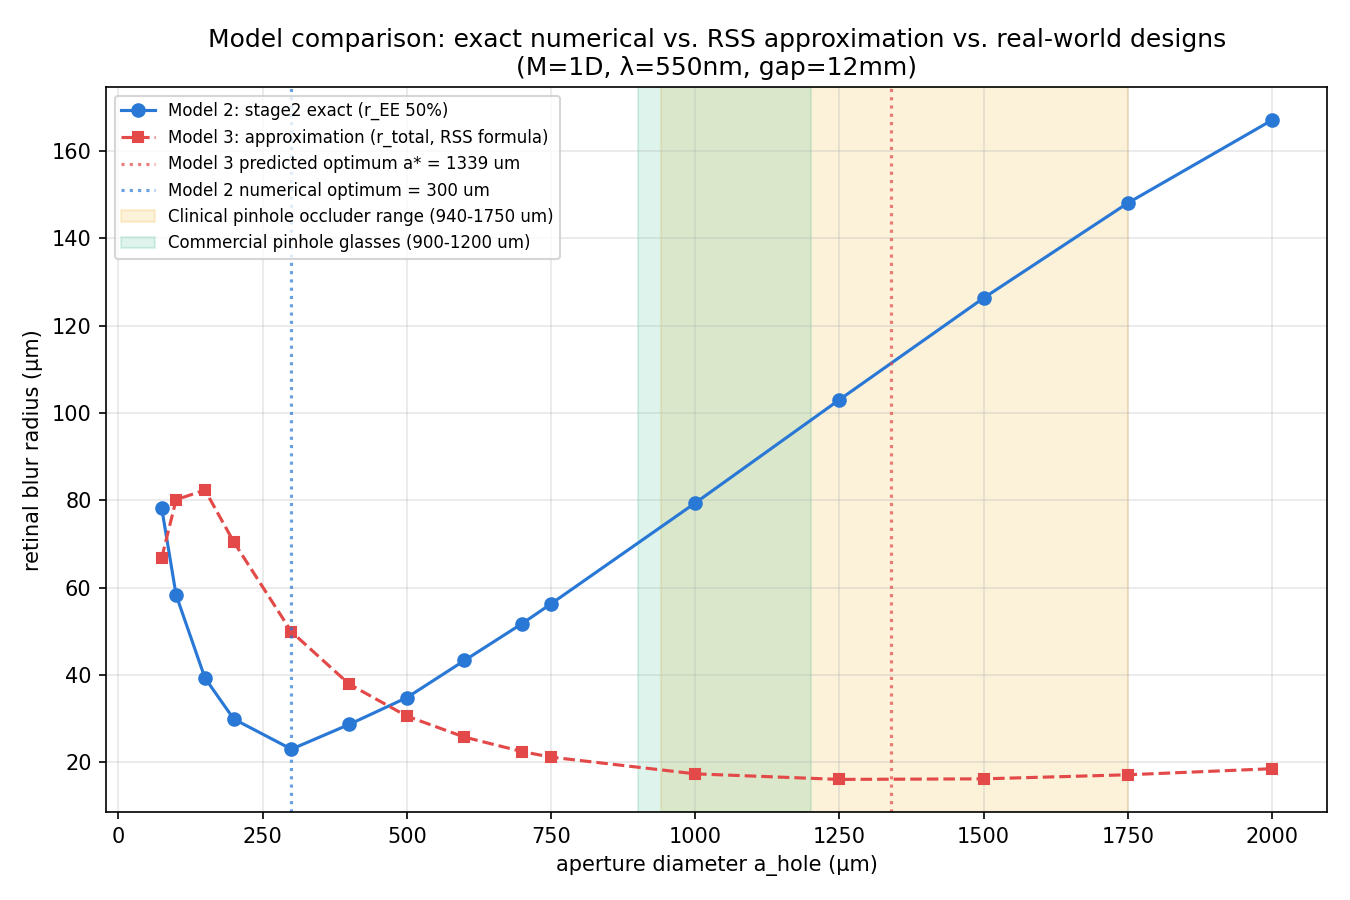
\includegraphics[width=0.8\textwidth]{figs/comparison_retina_M1.png}
\caption{Retina-plane, $M=1$D: old RSS $\rtotal$ vs.\ exact $r_{EE}(50\%)$. Divergence worst at mild myopia.}
\label{fig:comp-m1}
\end{figure}
\begin{figure}[h!]
\centering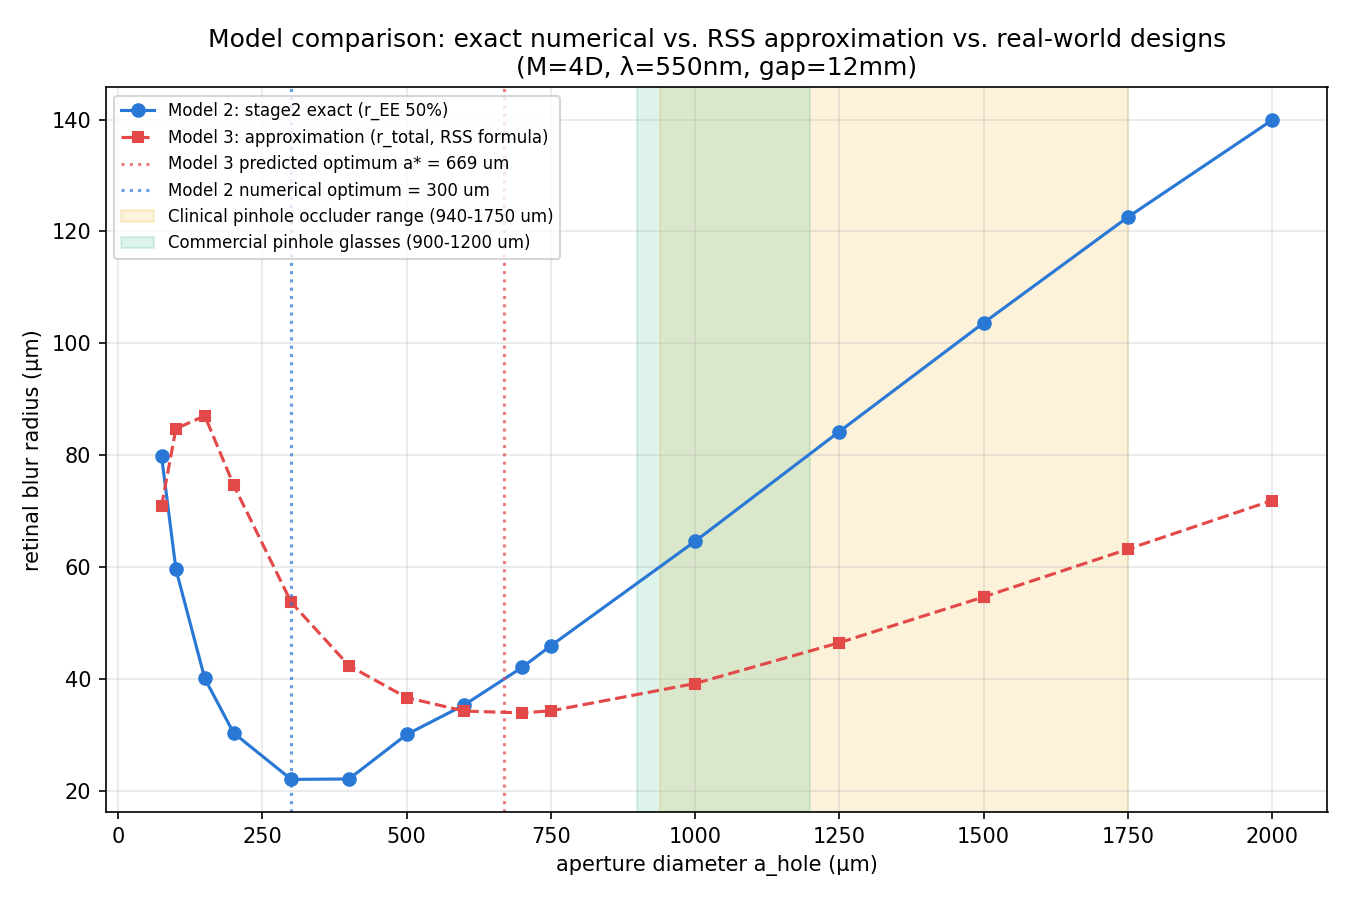
\includegraphics[width=0.8\textwidth]{figs/comparison_retina_M4.png}
\caption{Retina-plane, $M=4$D. Note the RSS formula's own spurious secondary dip near $100$--$150\,\mu$m.}
\label{fig:comp-m4}
\end{figure}
\begin{figure}[h!]
\centering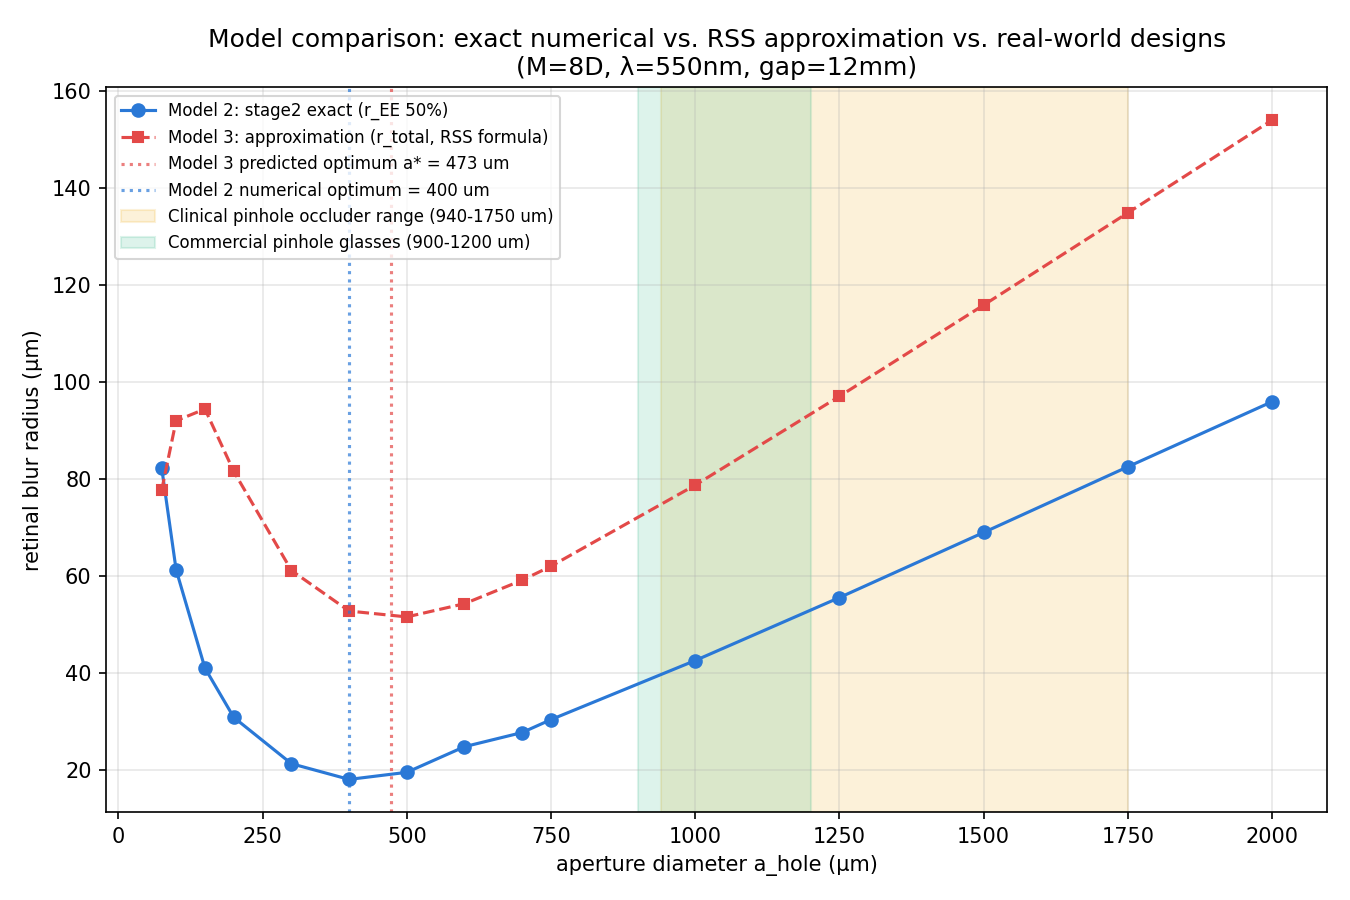
\includegraphics[width=0.8\textwidth]{figs/comparison_retina_M8.png}
\caption{Retina-plane, $M=8$D. Divergence narrows at higher myopia but remains large.}
\label{fig:comp-m8}
\end{figure}

\textbf{Root cause}, confirmed by direct calculation: $\aeff$ (Eq.~\ref{eq:aeff}) is itself non-monotonic at small apertures, producing a spurious secondary dip around $100$--$150\,\mu$m unrelated to the true optimum.

\section{Finding 2 --- none of the three physics models land near commercial/clinical designs}
\begin{table}[h!]
\centering
\caption{Reference apertures: this project's models vs.\ independent literature.}
\begin{tabular}{lc}
\toprule
Source & Aperture diameter \\
\midrule
Model 2 (this project, $r_{EE}$ 50\%) & $300$--$400\,\mu$m \\
Model 3 (closed-form $a^*$) & $473$--$1339\,\mu$m \\
Rayleigh pinhole-camera formula, $d=1.9\sqrt{f\lambda}$ & $210$--$225\,\mu$m \\
Clinical pinhole occluders (optometry) & $940$--$1750\,\mu$m ($\sim1200\,\mu$m typical) \\
Commercial pinhole glasses & $900$--$1200\,\mu$m \\
\bottomrule
\end{tabular}
\end{table}

\begin{figure}[h!]
\centering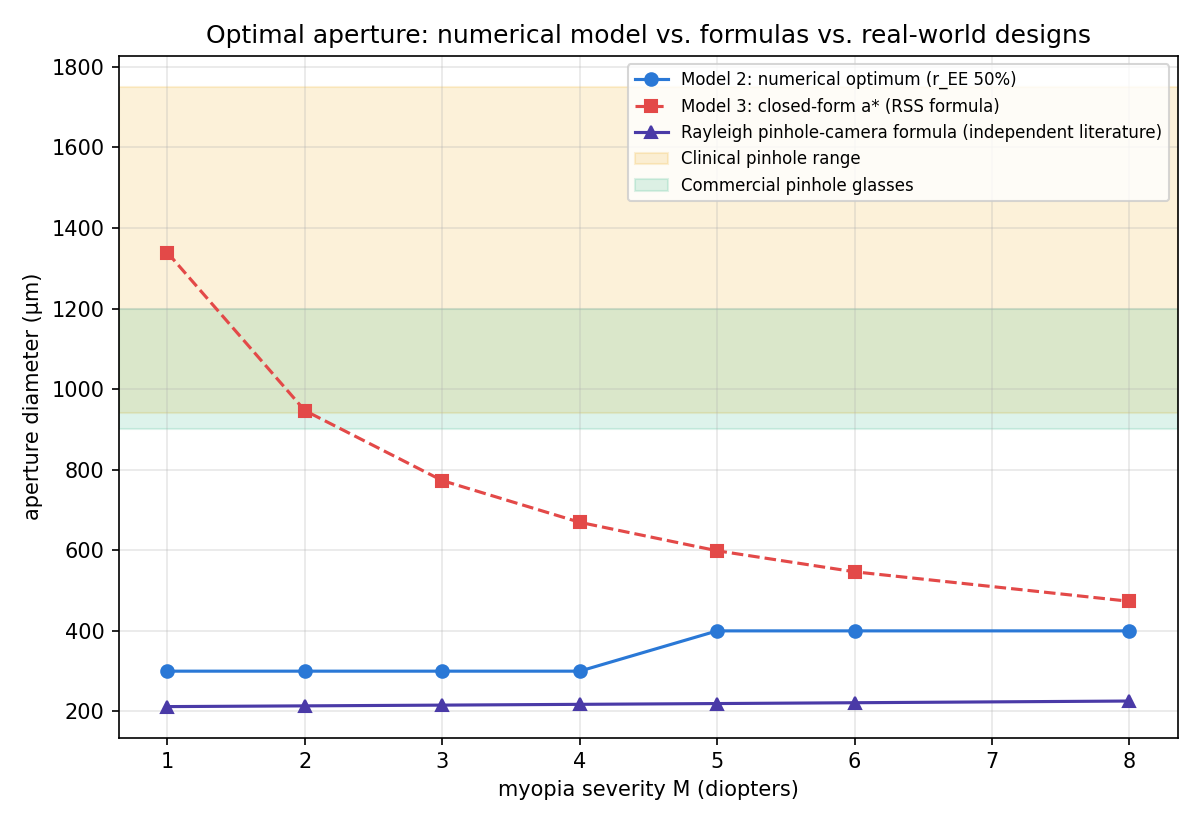
\includegraphics[width=0.8\textwidth]{figs/comparison_optimum_vs_rayleigh.png}
\caption{All five reference points: this project's two models, the independent Rayleigh formula, and the clinical/commercial range.}
\end{figure}

All three physics-based results cluster in the $200$--$700\,\mu$m range -- consistently smaller than any commercial or clinical product. The diagnosed explanation is scope, not error: every physics model here optimizes blur alone. A $300\,\mu$m hole passes roughly $16\times$ less light than a $1.2$mm hole (power $\propto d^2$), and no compared model builds in throughput or usability constraints. Chapter~\ref{ch:stage3a}'s brightness-constrained result is exactly the corrective step this finding calls for.

\section{Finding 3 --- a genuine metric-selection error, confirmed against a real clinical study}
\label{sec:finding3}
Applying Eq.~\ref{eq:acuityliteral} literally, using $r_{EE}(50\%)$, at the same condition a real clinical study measured ($1.2$mm aperture, $\sim5$D myopia, reported $\sim20/30$ Snellen, $0.17$ logMAR):

\begin{table}[h!]
\centering
\caption{Acuity metric comparison against a real clinical data point.}
\begin{tabular}{lccc}
\toprule
Metric & Value & Implied blur & Implied Snellen \\
\midrule
$r_{EE}(50\%)$ & $73.8\,\mu$m & $10.45$ arcmin & $\sim 20/209$ \\
FWHM (core-width) & $16.9\,\mu$m & $2.39$ arcmin & $\sim 20/48$ \\
\bottomrule
\end{tabular}
\end{table}

$r_{EE}(50\%)$ predicts acuity nearly \textbf{seven times worse} than the clinical measurement. FWHM lands within roughly $1.6\times$. Mechanism: $r_{EE}(50\%)$ is a cumulative-\emph{energy} radius, counting diffuse peripheral light in faint outer Fresnel rings that does not meaningfully impair letter recognition, while FWHM measures only the bright, legibility-relevant core.

This does not mean $r_{EE}(P)$ is wrong everywhere -- for the blur-distribution objective it is exactly what the reference handbooks specify. It is specifically wrong when repurposed, unmodified, for an acuity claim. \textbf{Any future acuity conversion should use a core-width metric, not $r_{EE}(50\%)$}, and should not be assumed accurate beyond a factor of roughly two given this project's scope (\S1.2).

\section{What this comparison does not claim}
This does not conclude the numerical models (Stages 1/2) are wrong. Every divergence has a specific, checked mechanism: RSS-vs-convolution (Finding 1), missing throughput/usability constraints (Finding 2), cumulative-energy-vs-core-width metric choice (Finding 3). No correction reconciles numbers to match a reference without first understanding why they differ.

\chapter{Patent and Real-World Literature Cross-Reference}
\label{sec:patents}

\section{Two patents examined directly}
\subsection{KR 10-2081511 (granted invention patent, 2020)}
Effective aperture: a funnel/cone hole, $0.9$mm at the eye-facing surface widening to $2.5$--$2.8$mm outer, with an asymmetric internal reflective coating eliminating a documented "haze" glare effect. The $0.9$mm figure sits almost exactly at the \emph{lower edge} of this project's verified clinical bracket -- a genuine convergence point, attributed to described inventor testing, not a cited acuity study; no brightness analysis appears in the patent.

\subsection{CN 201716487U (utility model, circa 2010--2011)}
Claims a five-hole cross array, main claim diameter $<0.8$mm, preferred embodiment $<0.4$mm -- genuinely close to this project's own blur-only result. The patent's background section justifies this on bare geometric-optics grounds (asserting $>1$mm holes "cannot form pinhole imaging"), with \emph{zero} brightness, illuminance, or clinical data anywhere in the document. A Chinese utility model is administratively registered, not substantively examined for novelty or function -- this patent's sub-$0.4$mm claim carries materially less evidentiary weight, and plausibly shares this project's own uncorrected blind spot.

\begin{table}[h!]
\centering
\caption{Patent dimension comparison, direct from source text.}
\begin{tabular}{p{4cm}p{4cm}p{4cm}}
\toprule
Parameter & KR 10-2081511 & CN 201716487U \\
\midrule
Patent type & Granted invention patent & Utility model (unexamined) \\
Effective diameter & $0.9$mm & $<0.8$mm ($<0.4$mm preferred) \\
Hole spacing & $3.2$--$4.8$mm & $0.7$--$1.2$mm \\
Stated basis & Inventor-described testing & Bare assertion, no testing \\
Brightness discussed? & No & No \\
Vs.\ clinical bracket & Lower edge (convergent) & Well below (divergent) \\
\bottomrule
\end{tabular}
\end{table}

\section{Evidentiary hierarchy}
Ranked strongest to weakest: (1) peer-reviewed clinical acuity studies; (2) the KR granted patent with described testing; (3) the CN utility model, an unexamined assertion sharing this project's own uncorrected blind spot.

\section{Cited real-world reference values}
\label{sec:clinicalbracket}
\begin{itemize}[leftmargin=1.2cm]
\item Clinical pinhole occluder diameter, effective range $0.94$--$1.75$mm, $\sim1.2$mm typical -- "A Peek at the Pinhole" (Review of Optometry); "The Ideal Pinhole" (IOVS/ARVO, 2009).
\item Commercial pinhole glasses: $\sim1.0$--$1.2$mm diameter, $2$--$4$mm spacing (myopia.org).
\item Clinical acuity data point: $1.2$mm aperture $\to$ $20/30$ Snellen ($0.17$ logMAR) up to $5.5$D myopia.
\item Rayleigh pinhole-camera formula, $d=k\sqrt{f\lambda}$, $k=1.9$ (Rayleigh's 1891 value).
\item MAR/Snellen conversion (StatPearls/NCBI).
\end{itemize}

\chapter{Error Budget and Uncertainty Analysis}
\label{ch:errorbudget}

\section{Validation statistics}
Numeric result vs.\ closed-form Airy formula, at the validation-gate configuration ($\ahole=150\,\mu$m, $550$nm, grid $N{=}4096$, window $6$mm):

\input{chapter9_validation_table.tex}

\section{Extended error budget}
\label{sec:errorbudget}
Every known contributor to the gap between this project's predictions and real human visual performance:

\input{chapter9_errorbudget_table.tex}

\section{Uncertainty propagation}
For every citation entry marked \emph{heuristic} or \emph{published-approximate}, its stated uncertainty range was propagated into the primary optimum-aperture number. Ocular transmission (heuristic default $0.90$, range $0.85$--$0.95$) does \emph{not} affect $r_{EE}(50\%)$ at all, since that metric is purely geometric/energy-based -- it only affects photometry-derived quantities (photon flux, $\sim11\%$ range at the reference $400\,\mu$m aperture). The CSF peak-location disagreement ($4$ vs.\ $8$ cycles/degree) is a genuine published-model disagreement, not an uncertainty band on one model.

\section{The two confirmed anomalies, restated}
Both anomalies (\S\ref{sec:anomaly1},\ref{sec:anomaly2}) are logged as quantified, project-original findings in the extended error budget above: retina-plane FWHM ring-hopping ($4.7\to154.7\,\mu$m jump) and Strehl non-monotonicity (confirmed genuine, up to $8.4\times$ swing).

\chapter{Open Items and Roadmap}
\label{ch:roadmap}

\section{What remains genuinely open}
\label{sec:openitems}
\begin{itemize}[leftmargin=1.2cm]
\item The $6$--$9\%$ brightness floor (\S\ref{sec:stage3aresult}) closes the gap in magnitude but was found by matching a known target, not derived from a cited photopic illuminance-acuity threshold. Locating such a citation is the highest-priority remaining task.
\item Retina-plane FWHM and Strehl ratio (both confirmed unstable) should not be used as primary design metrics without further work.
\item Only a single circular aperture is modeled. Real pinhole eyewear (and both examined patents) uses multi-hole arrays; Eq.~\ref{eq:ghosting}--\ref{eq:photometryarray} are derived but not yet simulated.
\item Polychromatic simulation exists only as a representative 3-wavelength subset; the full incoherent-sum composite (per the polychromatic note, \S\ref{ch:formulas}) remains undone.
\item No higher-order ocular aberrations, accommodation, fixational eye movements, or Stiles--Crawford apodization are modeled anywhere (\S1.2, \S\ref{sec:errorbudget}).
\end{itemize}

\section{The deliberate decision to defer empirical validation}
This handbook does not put forward one final recommended aperture -- a considered decision, not an omission. Theory can narrow the design space and bound plausible mechanisms; it cannot substitute for a genuinely empirical fact about a nonlinear biological visual system at a given brightness level. The recommended next step: a physical pinhole test rig (real apertures at, e.g., $300,500,700,900,1200,1500\,\mu$m; fixed measured ambient brightness; Snellen/logMAR chart; real myopic subjects or simulated myopia via a known defocus lens, mapping directly onto this project's own $M$ axis).

\section{Interactive exploration tools built alongside this handbook}
A live parameter-exploration Streamlit tool (adjustable aperture, wavelength, myopia, gap, pupil diameter, brightness floor, with cached fast-preview and explicit high-accuracy modes never conflated) and a four-tab flagship application (adding a letter-chart blur animation, a browser for this handbook's precomputed outputs, and a persistent session log) were specified -- explicitly scoped as exploration/data-collection tools, with no single-recommended-aperture output built into either, by design.

\chapter{Conclusion}

This handbook consolidates a genuinely deep body of work distinguished by three things. First, every gap between models was diagnosed to a specific, checked mechanism rather than ignored or silently reconciled -- the RSS formula's failure (mean $64.8\%$, max $192.8\%$), the brightness-constraint explanation for the commercial-product gap (quantitatively closing it at a $6$--$9\%$ floor), and the $r_{EE}(50\%)$-vs-FWHM acuity metric error (confirmed against a real clinical study, not merely asserted).

Second, two genuine anomalies -- retina-plane FWHM ring-hopping and Strehl non-monotonicity -- were investigated rather than assumed away, and both confirmed as real physical behavior via a tenfold finer sweep that made the effect \emph{more} pronounced, the signature of genuine structure rather than sampling noise.

Third, and most importantly, this handbook stops short of manufacturing false certainty. It does not report one final recommended aperture. The brightness-corrected theoretical prediction ($900$--$1250\,\mu$m) is presented as consistent with, but not proven equal to, the real clinical and commercial range, and the most load-bearing number in reaching that conclusion (the $6$--$9\%$ brightness floor) is explicitly flagged as reverse-engineered rather than independently derived. The path forward is concrete: locate an independent illuminance-acuity citation, build the multi-hole array and no-ghost constraints already derived but not simulated, complete the polychromatic pass, and build the physical test rig that can answer the one question no further simulation can settle alone -- what a real human eye, at a real brightness level, actually resolves through a real pinhole.

\appendix
\chapter{Full Literature Citation Database}
\label{app:literature}
Rendered directly from \texttt{literature.py}'s own \texttt{CITATIONS} dictionary (Stage 3 Human Vision) so this table can never drift out of sync with the source code that uses it.

\input{appendixA_table.tex}

\chapter{Module and Code Inventory}
\label{app:modules}

\section*{stage1\_v2/ (cornea-plane diffraction)}
\texttt{physics.py}: \texttt{make\_grid}, \texttt{circular\_aperture}, \texttt{asm\_transfer\_function}, \texttt{asm\_propagate}, \texttt{precompute\_transfer\_function}, \texttt{fresnel\_number}, \texttt{fresnel\_regime}, \texttt{choose\_radial\_bins}, \texttt{radial\_profile}, \texttt{encircled\_energy}, \texttt{r\_for\_EE}, \texttt{second\_moment\_radius}, \texttt{locate\_threshold\_crossing}, \texttt{effective\_radius}/\texttt{effective\_radius\_detail}, \texttt{RunConfig}.

\section*{stage2/ and stage2\_fixed/ (full eye model)}
\texttt{myopia\_axial.py}: \texttt{axial\_length\_for\_myopia}. \texttt{pipeline\_junction.py}: \texttt{run\_gap\_to\_cornea}, \texttt{validate\_junction} (bug-fixed). \texttt{phase2\_retina.py}: \texttt{pupil\_clip}, \texttt{lens\_phase}, \texttt{propagate\_to\_retina}, \texttt{retinal\_encircled\_energy}, \texttt{run\_pipeline\_point}. \texttt{validation\_gate.py}: \texttt{airy\_EE}, \texttt{airy\_radius\_for\_EE}, \texttt{run\_validation\_gate}. \texttt{sweep\_myopia.py}: \texttt{build\_row}, \texttt{finalize\_row} (bug-fixed), \texttt{run\_sweep}. \texttt{classical\_formulas.py}: the deprecated $\aeff$/$\rgeo$/$\rdiff$/$\rtotal$/$a^*$ chain.

\section*{stage3a/ (brightness-constrained optimum)}
\texttt{transmission.py}: \texttt{relative\_illuminance}. \texttt{combine\_and\_select.py}: the $\Tmin$-constrained argmin sweep and figure generation.

\section*{stage3\_human\_vision/ (comprehensive metric suite)}
\texttt{literature.py}: the 20-entry citation database. \texttt{photometry.py}: \texttt{nearest\_v\_lambda}, \texttt{photon\_energy}, \texttt{radiance\_from\_luminance}, \texttt{retinal\_illuminance\_troland}, \texttt{relative\_retinal\_illuminance}, \texttt{retinal\_irradiance}, \texttt{photon\_flux\_at\_retina}. Plus \texttt{metrics.py}, \texttt{contrast.py}, \texttt{visual\_acuity.py}, \texttt{pareto.py}, \texttt{validation.py}, \texttt{comparison.py}, \texttt{plots.py}, \texttt{run\_metrics\_sweep.py}, \texttt{run\_stage3.py}.

\section*{stage3\_integrated/ (cross-validated merge)}
\texttt{combine\_metrics.py}: \texttt{build\_combined\_grid}, \texttt{constrained\_optimum\_all\_metrics}. \texttt{run\_full\_theory\_sweep.py}: \texttt{retina\_plane\_fwhm}, \texttt{sweep\_1\_retina\_fwhm}, \texttt{sweep\_2\_fine\_strehl}, \texttt{sweep\_3\_wavelength\_gap}. \texttt{generate\_plots.py}: ten plotting functions. \texttt{generate\_tables.py}: \texttt{table\_literature\_citations}, \texttt{table\_validation\_statistics}, \texttt{table\_uncertainty\_propagation}, \texttt{table\_error\_budget\_extended}.

\section*{model\_comparison/ (independent cross-check)}
\texttt{stage1\_runner.py}, \texttt{stage2\_runner.py}, \texttt{approximation\_runner.py}: thin wrappers reusing rather than reimplementing the compared models' physics. \texttt{run\_comparison.py}, \texttt{plot\_comparison.py}, \texttt{acuity\_check.py}: the Chapter~\ref{ch:comparison} findings.

\chapter{Symbol Table}
\label{app:symbols}
\begin{longtable}{p{2.3cm}p{8cm}p{2cm}}
\caption{Symbol table, reproduced from the project's reference handbooks and extended with symbols this handbook introduces.}\\
\toprule
\textbf{Symbol} & \textbf{Meaning} & \textbf{Unit} \\
\midrule
\endhead
$\ahole$ & physical pinhole diameter & m \\
$\aeff$ & effective spot diameter after gap propagation (deprecated) & m \\
$\astop$ & effective aperture stop after pupil clipping & m \\
$\dgap$ & pinhole film to cornea distance & m \\
$\vr$ & lens-to-retina distance & m \\
$\vf$ & lens-to-actual-focus distance & m \\
$u$ & object distance & m \\
$f$ & eye's pathological focal length & m \\
$\lambda$ & wavelength & m \\
$N_F$ & Fresnel number & --- \\
$\rgeo$ & geometric blur radius & m \\
$\rdiff$ & diffraction first-null radius & m \\
$r_{EE}(P)$ & radius enclosing energy fraction $P$ & m \\
$EE(x)$ & encircled energy function & --- \\
$N$ & hole count (array context) & --- \\
$s$ & hole pitch & m \\
$T$ & open-area transmission fraction & --- \\
$M$ & myopia magnitude & D (m$^{-1}$) \\
$\varphi$ & eye gaze rotation angle & rad/deg \\
$R_{\text{rot}}$ & center-of-rotation to pupil-plane distance & m \\
$t$ & film substrate thickness & m \\
$R_p, R_h$ & pupil, hole radii & m \\
$P_0$ & emmetropic eye optical power (default $60$D) & D \\
$n'$ & vitreous refractive index (default $1.336$) & --- \\
$L_0$ & emmetropic axial length, $n'/P_0$ & m \\
$L_{\text{ax}}$ & myopic axial length, $n'/(P_0-M)$ & m \\
$\Dpupil$ & natural pupil diameter (default $4000\,\mu$m) & m \\
$\Erel$ & relative retinal illuminance vs.\ full natural pupil & --- \\
$\Tmin$ & minimum acceptable relative illuminance (brightness floor) & --- \\
\bottomrule
\end{longtable}

\chapter{Full Constrained-Optimum-by-Metric Table}
\label{app:fulldata}
The complete brightness-constrained optimum aperture, by myopia level and brightness floor $\Tmin$, across five representative metrics of the ten computed in Stage 3 Integrated. This is the underlying data behind \S\ref{sec:convergence}'s convergence finding: at $\Tmin$ at or above roughly $6.25\%$, all metrics converge to the same optimum aperture per myopia level, regardless of which metric is used.

\input{appendixD_table.tex}

\chapter{Glossary of Terms}
\label{app:glossary}

\textbf{Angular Spectrum Method (ASM).} An exact numerical technique for propagating a wave field a given distance by decomposing it into plane waves, advancing each by its own propagation phase, and reassembling the result. Unlike Fresnel/Fraunhofer approximations, it makes no assumption about propagation distance relative to aperture size.

\textbf{Fresnel number ($N_F$).} A dimensionless number classifying diffraction regime (Eq.~\ref{eq:fresnelnumber}): $\ll 1$ far-field, $\sim1$--$10$ near-field transition, $\gg10$ near-geometric.

\textbf{Encircled energy, $r_{EE}(P)$.} The radius containing a specified fraction $P$ of total light power. Large-$P$ values can be substantially larger than the visually dominant central spot, due to faint outer diffraction rings.

\textbf{FWHM.} The diameter over which intensity stays above half its peak -- a core-width measure, ignoring peripheral rings entirely.

\textbf{MTF/OTF.} A description of contrast preservation vs.\ spatial frequency (Eq.~\ref{eq:mtfotf}), rather than a single blur radius.

\textbf{CSF.} Human contrast sensitivity vs.\ spatial frequency, peaking in a mid-range (reported between roughly $2$ and $8$ cycles/degree depending on model).

\textbf{Strehl ratio.} Ratio of actual to diffraction-limited peak intensity (Eq.~\ref{eq:strehl}); the Mar\'echal criterion treats $0.8$ as the diffraction-limited threshold.

\textbf{RSS vs.\ convolution.} RSS combines blur radii as $\sqrt{r_1^2+r_2^2}$ -- simple but not physically correct; the correct combination convolves point-spread functions.

\textbf{Troland (Td).} Standard unit of retinal illuminance: illuminance from a $1\,\text{cd/m}^2$ surface through a $1\,\text{mm}^2$ pupil.

\textbf{Pareto front.} The set of designs where no objective can improve without another worsening.

\textbf{Snellen / logMAR / MAR.} Snellen acuity (e.g.\ $20/20$) as a resolution-distance ratio; MAR is the angular size of the smallest resolvable detail in arcminutes ($20/20 = 1$ arcmin); logMAR is $\log_{10}(\text{MAR})$.

\textbf{Diopter (D).} Reciprocal focal length in meters; myopia severity is conventionally expressed in diopters.

\chapter{Reproducibility: Exact Commands per Stage}
\label{app:reproduce}
Every figure, table, and number in this handbook traces to a specific script. This appendix lists the exact command to regenerate each stage's output from scratch.

\section*{Stage 1}
\texttt{python3 sweep.py}

\section*{Stage 2}
\texttt{python3 validation\_gate.py}\\
\texttt{python3 sweep\_myopia.py --a-hole-um 75,100,...,2000 --M-diopters 1,2,3,4,5,6,8 \textbackslash} \\
\texttt{\ \ --wavelengths-nm 450,550,650 --d-gap-mm 12,15}

\section*{Stage 3a}
\texttt{python3 combine\_and\_select.py} \\
\texttt{python3 plot\_blur\_then\_constraint.py --T-min 0.0625}

\section*{Stage 3 Human Vision}
\texttt{python3 run\_stage3.py} \\
\texttt{python3 run\_metrics\_sweep.py} \\
\texttt{python3 literature.py}

\section*{Stage 3 Integrated}
\texttt{python3 combine\_metrics.py} \\
\texttt{python3 run\_full\_theory\_sweep.py all} \\
\texttt{python3 generate\_plots.py} \\
\texttt{python3 generate\_tables.py}

\section*{Model Comparison}
\texttt{python3 run\_comparison.py} \\
\texttt{python3 plot\_comparison.py} \\
\texttt{python3 acuity\_check.py}

\end{document}
